\documentclass[10pt,a4paper]{article}

\usepackage[margin=16mm,top=15mm,bottom=17mm]{geometry}
\usepackage{kotex}
\usepackage{amsmath,amssymb}
\usepackage{graphicx}
\usepackage{booktabs}
\usepackage{tabularx}
\usepackage{array}
\usepackage{enumitem}
\usepackage{caption}
\usepackage{subcaption}
\usepackage{float}
\usepackage{placeins}
\usepackage{xcolor}
\usepackage{listings}
\usepackage[hidelinks]{hyperref}

\setmainfont[
    Path=/usr/share/fonts/truetype/unfonts-core/,
    UprightFont=UnBatang.ttf,
    BoldFont=UnBatangBold.ttf,
    Ligatures=TeX
]{UnBatang}
\setmainhangulfont[
    Path=/usr/share/fonts/truetype/unfonts-core/,
    UprightFont=UnBatang.ttf,
    BoldFont=UnBatangBold.ttf
]{UnBatang}

\graphicspath{{./}{reports/}}
\renewcommand{\thesubsection}{\thesection-\arabic{subsection}}
\captionsetup{font=small,labelfont=bf}
\setlist[itemize]{leftmargin=*,topsep=2pt,itemsep=1pt}
\setlist[enumerate]{leftmargin=*,topsep=2pt,itemsep=1pt}
\renewcommand{\arraystretch}{1.13}
\setlength{\parindent}{0pt}
\setlength{\parskip}{4pt}

\definecolor{deepblue}{HTML}{1D4ED8}
\definecolor{softgray}{HTML}{F8FAFC}
\definecolor{rulegray}{HTML}{CBD5E1}
\definecolor{darkgray}{HTML}{334155}
\newcolumntype{Y}{>{\raggedright\arraybackslash}X}
\newcommand{\placeholder}[1]{\textcolor{gray}{(#1)}}
\newcommand{\code}[1]{\texttt{#1}}

\lstdefinestyle{pseudo}{
    basicstyle=\ttfamily\footnotesize,
    keywordstyle=\bfseries\color{deepblue},
    commentstyle=\itshape\color{darkgray},
    frame=single,
    rulecolor=\color{rulegray},
    backgroundcolor=\color{softgray},
    columns=fullflexible,
    keepspaces=true,
    showstringspaces=false,
    breaklines=true,
    tabsize=2,
    xleftmargin=2mm,
    xrightmargin=2mm,
    numbers=left,
    numberstyle=\tiny\color{darkgray},
}

\begin{document}

\section{전체 시스템의 개요}
\subsection{로봇항공기(드론) 전체 시스템에 대한 설명}

대회 임무는 GPS 사용 없이 2m 고도에서 바닥 구획선을 따라 이동하고, 24m $\times$ 15m 격자 구역의 교차점에 무작위로 배치된 ArUco 경로점 4개를 탐색한 뒤, 식별번호 역순으로 재방문하는 것이다. 본 팀은 기체 형상 자체보다 \textbf{GPS 비의존 항법, 경로 비용 모델, 인식 연동 Offboard 제어}를 자체 개발 범위로 정의한다.

\begin{table}[H]
\centering
\small
\caption{규정 및 설계 기준 파라미터}
\begin{tabularx}{\linewidth}{p{34mm}p{34mm}Y}
\toprule
\textbf{항목} & \textbf{값} & \textbf{설계 반영}\\
\midrule
안전구역 / 미션구역 & 32m $\times$ 23m / 24m $\times$ 15m & Gazebo world와 경로 plotter의 좌표계 기준\\
격자 및 교차점 & 3m 간격, 9 $\times$ 6 = 54개 & Phase 1 탐색 후보 및 위치 snap 기준\\
ArUco 마커 & 4개, 0.5m $\times$ 0.5m & 하향 카메라 검출 및 confidence filter 대상\\
비행 고도 & 지면 기준 2m & ToF/기압계/PX4 고도 제어 목표\\
탐색 호버링 & 최초 인식 마커마다 3초 & \code{HOVER\_CONFIRM} 상태와 cost model에 반영\\
구조 경로 & 식별번호 역순, 구획선 추종 미검증 & ID 내림차순 직선 스프린트 경로 생성\\
\bottomrule
\end{tabularx}
\end{table}

\begin{figure}[H]
\centering
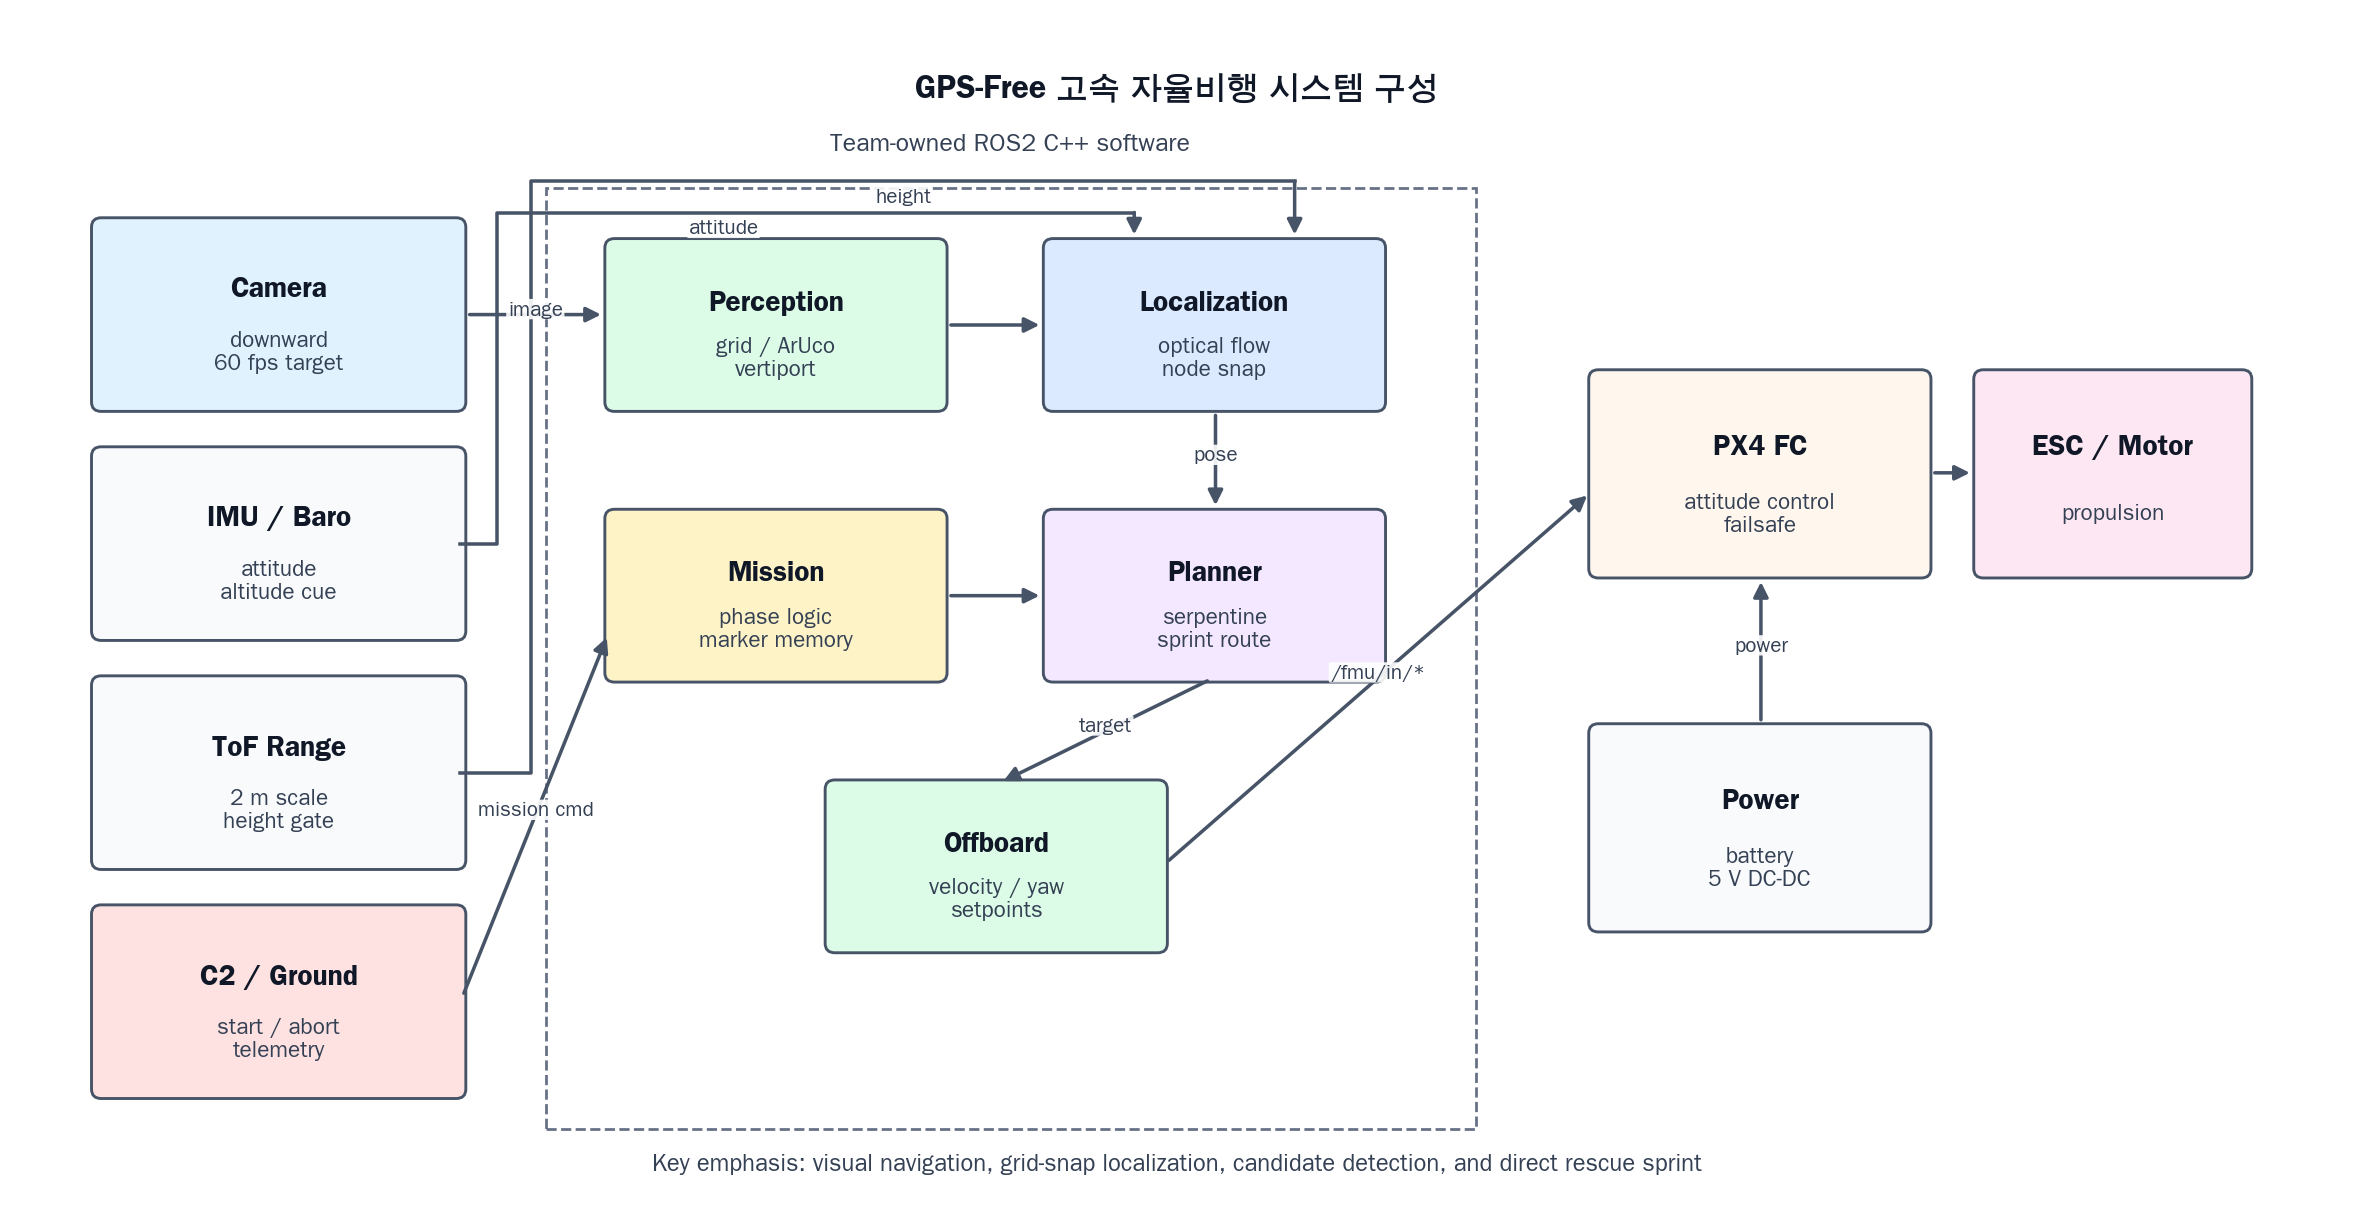
\includegraphics[width=0.93\linewidth]{fig_01_system_block.png}
\caption{GPS 비의존 자율비행을 위한 전체 시스템 블록도. 하향 카메라, IMU, ToF 입력을 ROS2 C++ 노드가 처리하고 PX4 Offboard setpoint로 변환한다.}
\end{figure}

운용 단계는 Fig. 2와 같이 Phase 0--3으로 구성한다. Phase 1에서는 교차점-to-교차점 S자 탐색을 수행하는 동안 하향 카메라 ArUco 검출을 계속 병행한다. 별도의 탐색 후 인식 단계가 있는 것이 아니라, 이동 중 마커 후보가 확정될 때만 같은 Phase 1 안에서 접근ㆍ흔들림 억제ㆍ3초 호버링 하위 상태로 전환한다. Phase 2에서는 구조 경로의 구획선 추종 미검증 조건을 활용하여 저장 좌표 사이를 직선으로 이동한다.

\begin{figure}[H]
\centering
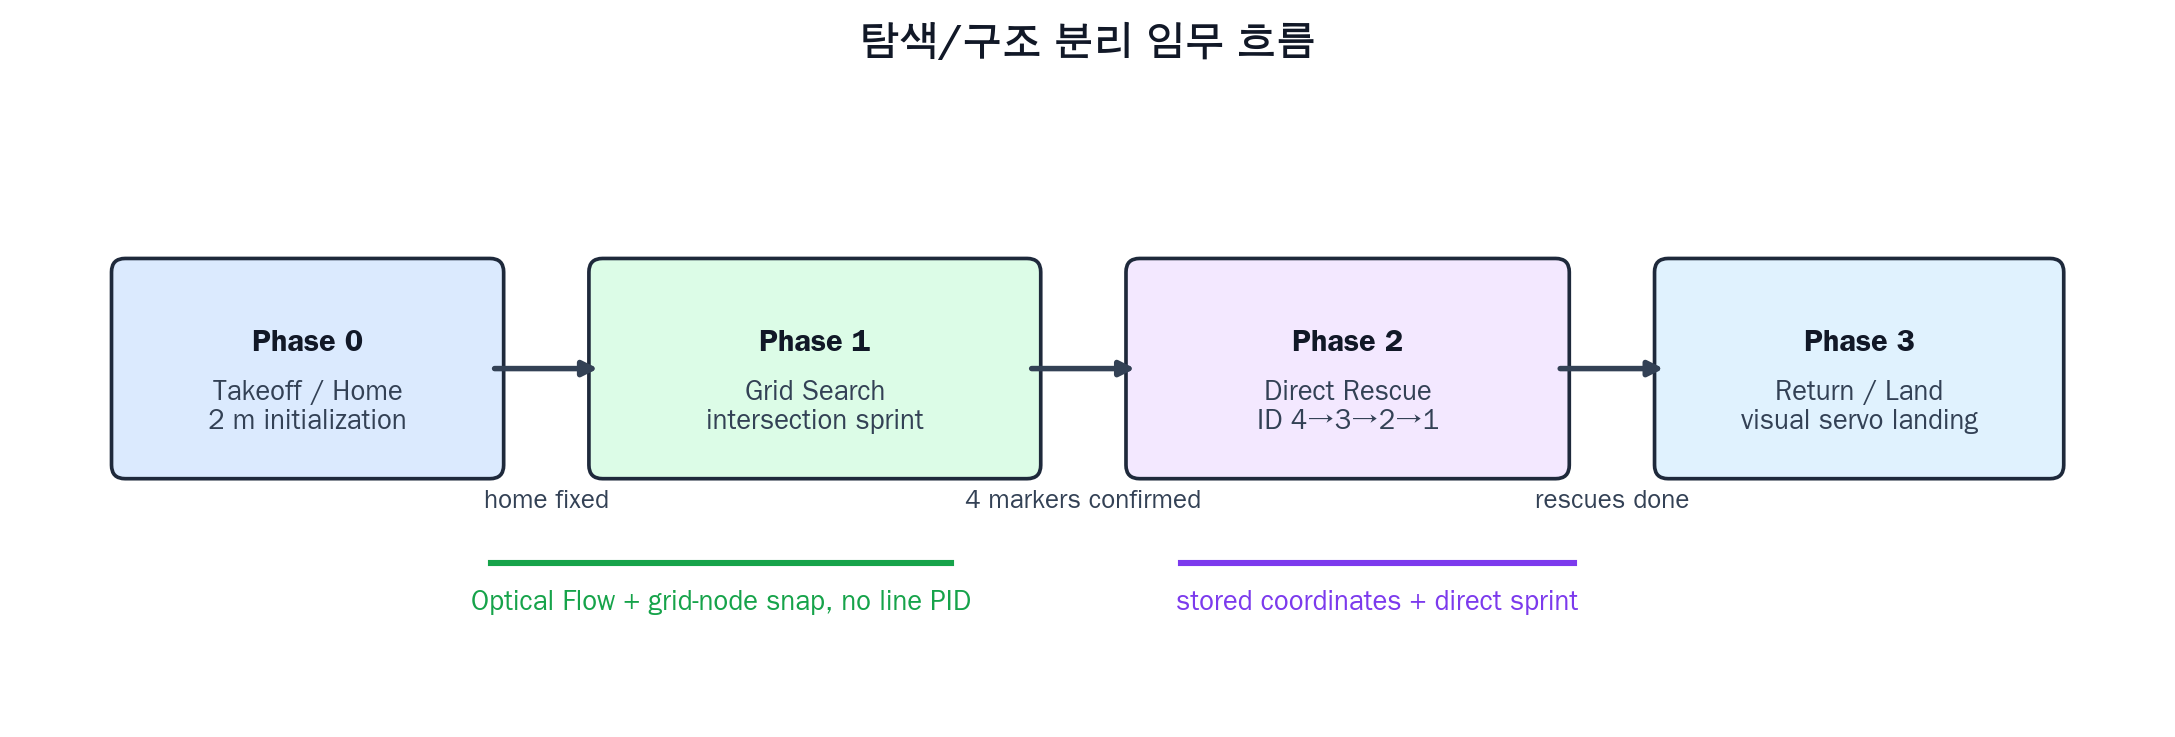
\includegraphics[width=0.96\linewidth]{fig_02_mission_flow.png}
\caption{Phase 0--3 미션 흐름. 탐색, 마커 저장, 구조 스프린트, 귀환/착륙을 상태 기계로 분리한다.}
\end{figure}

\section{자동비행 시스템 및 구현 기술}
\subsection{유도, 제어, 항법시스템 설계}

\textbf{항법 모델.} 하향 카메라의 프레임 간 픽셀 이동량을 ToF 고도와 카메라 화각으로 실제 이동량으로 환산한다. 영상 폭을 $W$, 수평 화각을 $\theta$, 고도를 $h_k$, 프레임 간 평균 픽셀 이동을 $(\Delta u_k,\Delta v_k)$, 시간 간격을 $\Delta t_k$라 하면 픽셀-미터 스케일과 기체 좌표계 속도는 다음과 같다.

\begin{equation}
s(h_k)=\frac{2h_k\tan(\theta/2)}{W},
\qquad
\mathbf{v}^{b}_k
=-\frac{s(h_k)}{\Delta t_k}
\begin{bmatrix}\Delta u_k\\ \Delta v_k\end{bmatrix}.
\end{equation}

IMU yaw $\psi_k$를 이용해 기체 좌표계 속도를 격자 좌표계로 회전하고 위치를 적분한다.

\begin{equation}
\hat{\mathbf{p}}_{k+1}^{-}
=\hat{\mathbf{p}}_{k}^{+}
+R(\psi_k)\mathbf{v}^{b}_k\Delta t_k,
\qquad
R(\psi)=
\begin{bmatrix}
\cos\psi & -\sin\psi\\
\sin\psi & \cos\psi
\end{bmatrix}.
\end{equation}

본 계획에서 Optical Flow는 라인 트래킹을 대체해 격자선을 더 정밀하게 따라가기 위한 알고리즘이 아니라, \textbf{교차점 사이 3m 구간을 빠르게 이동하는 동안의 거리 추정 계층}이다. 전통적인 라인 PID는 카메라 영상에서 선 중심과 방향을 매 프레임 안정적으로 유지해야 하므로 저속 구획선 추종에는 유리하지만, 교차점이 반복되는 격자에서는 분기점 판단과 yaw 정렬 때문에 속도를 보수적으로 잡게 된다. 반면 본 전략은 교차점 좌표를 목표점으로 두고, 교차점 사이에서는 Optical Flow/IMU/ToF로 상대 이동량을 추정한 뒤 다음 교차점에서 위치를 다시 snap한다. 따라서 라인은 ``계속 물고 가는 대상''이 아니라 3m마다 drift를 제한하는 절대 보정 기준으로 사용된다.

\begin{table}[H]
\centering
\small
\caption{격자 환경에서 라인 트래킹과 Optical Flow+교차점 snap의 역할 비교}
\begin{tabularx}{\linewidth}{p{28mm}Y Y}
\toprule
\textbf{항목} & \textbf{라인 트래킹 중심 접근} & \textbf{본 계획의 Optical Flow+snap 접근}\\
\midrule
제어 기준 & 선 중심/방향을 매 프레임 추종 & 교차점 좌표를 목표로 이동량 적분 후 3m마다 보정\\
격자 교차점 처리 & 분기점에서 선 선택과 yaw 정렬 필요 & 가장 가까운 격자 노드로 위치 snap 후 다음 목표 선택\\
속도 영향 & 영상 blur, 선 끊김, 급회전 때문에 보수적 속도 설정 & 교차점 사이 일시적 선 손실을 허용하고 정지 횟수 최소화\\
주요 리스크 & 선 추종 안정성은 높지만 시간 손실 가능 & Optical Flow drift가 존재하므로 교차점 검출과 snap 검증 필요\\
\bottomrule
\end{tabularx}
\end{table}

Optical Flow는 적분 오차가 누적되므로, 교차점 검출 시 가장 가까운 격자 노드 $\mathbf{g}_i$로 위치를 보정한다. $d_i=\lVert \hat{\mathbf{p}}_{k}^{-}-\mathbf{g}_i\rVert$이고 snap 반경이 $r_s$일 때,

\begin{equation}
\hat{\mathbf{p}}_{k}^{+}=
\begin{cases}
\mathbf{g}_{i^\star}, & i^\star=\arg\min_i d_i,\ d_{i^\star}<r_s,\\
\hat{\mathbf{p}}_{k}^{-}, & \text{otherwise}.
\end{cases}
\end{equation}

\begin{figure}[H]
\centering
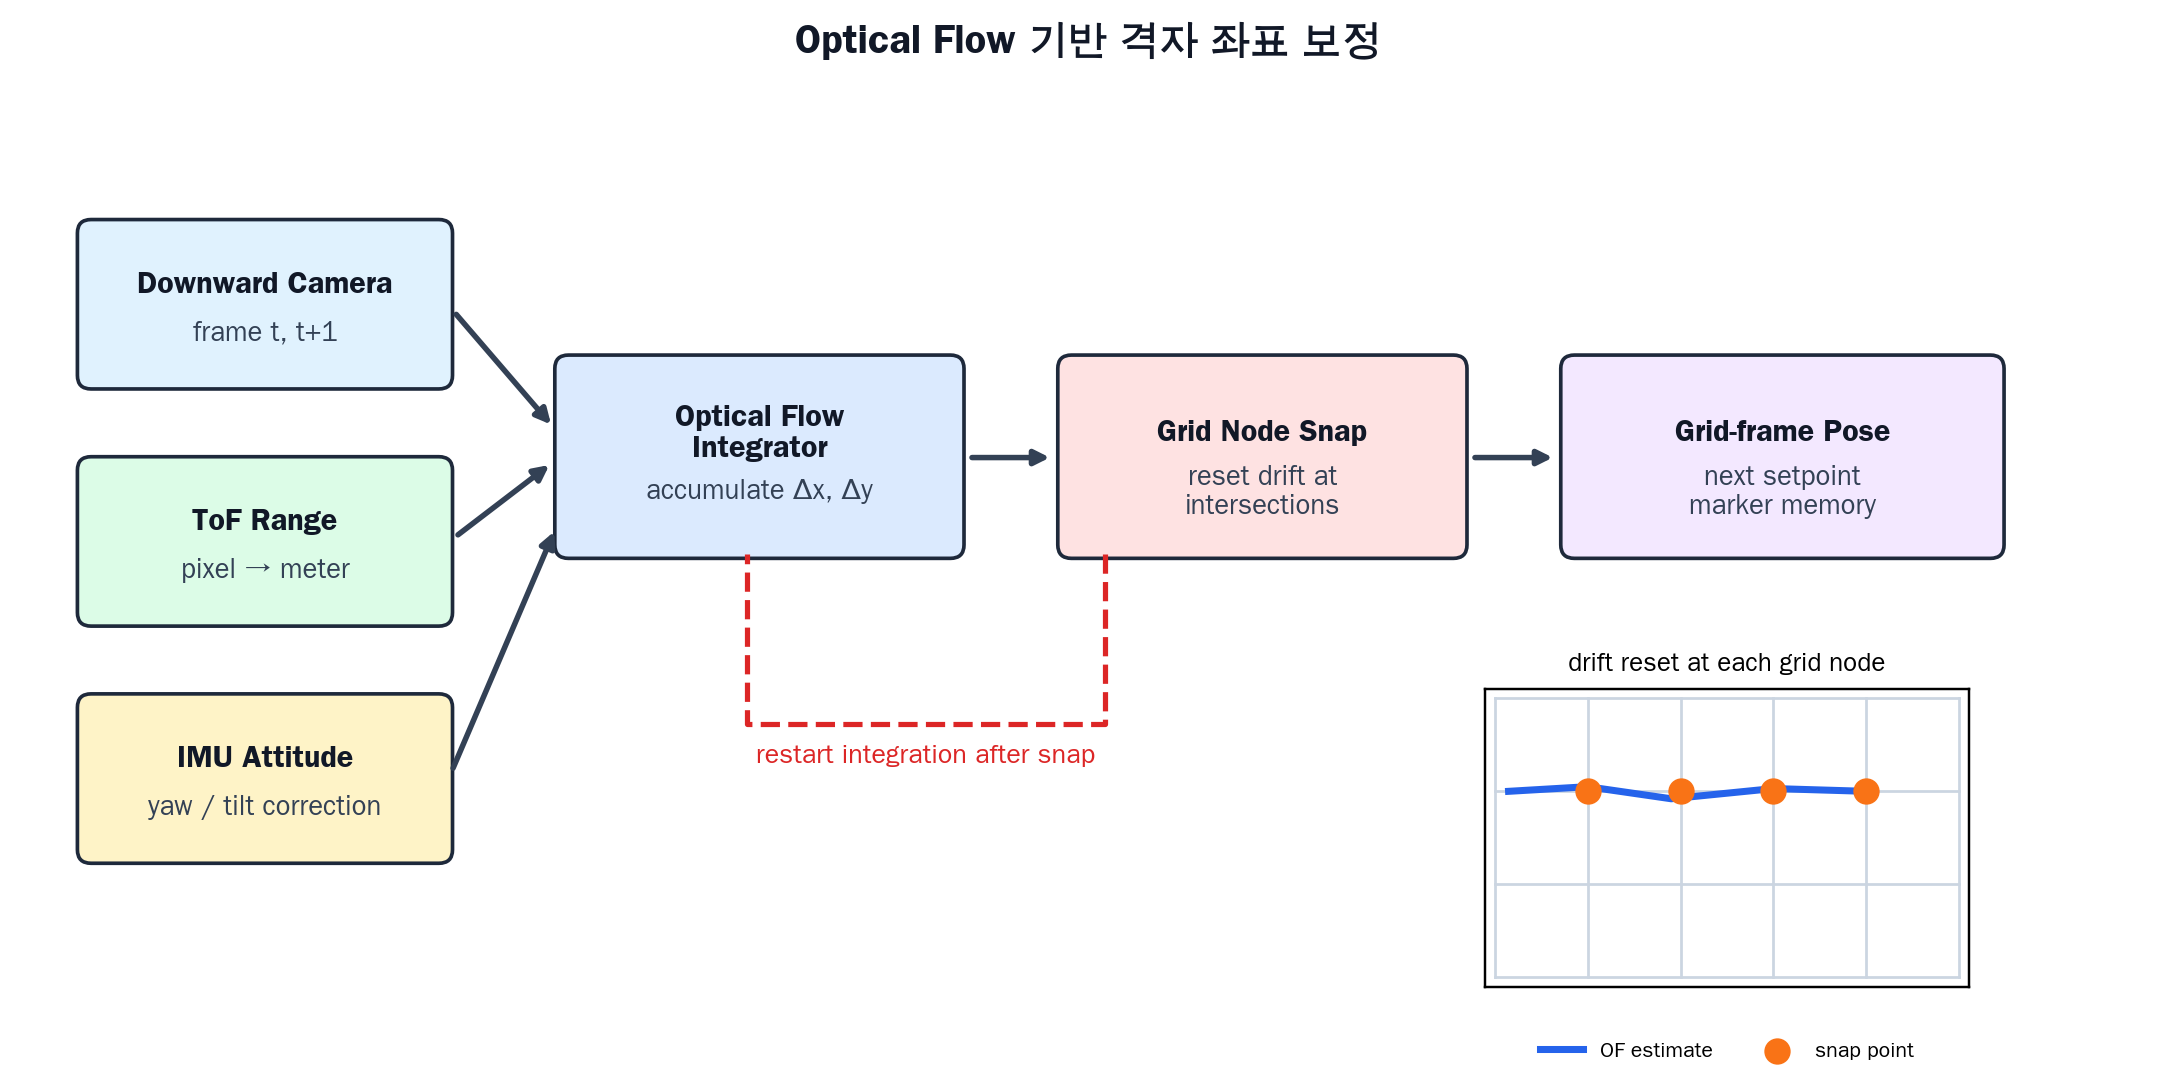
\includegraphics[width=0.84\linewidth]{fig_03_optical_flow_snap.png}
\caption{Optical Flow, ToF 고도 스케일, IMU yaw 보정, 교차점 snap을 결합한 위치 추정 구조.}
\end{figure}

\textbf{ArUco confidence filter.} 마커 검출은 단일 프레임 판정이 아니라 ID별 상태량 $c_i\in[0,1]$을 누적한다. 관측이 안정적이면 confidence를 증가시키고, 흔들림 또는 누락 프레임에서는 감쇠한다.

\begin{equation}
c_{i,k}=
\begin{cases}
\min(1,c_{i,k-1}+\alpha q_k), & \text{stable observation},\\
\min(1,\lambda c_{i,k-1}+0.5\alpha q_k), & \text{unstable observation},\\
\mu c_{i,k-1}, & \text{missing observation},
\end{cases}
\end{equation}
여기서 $q_k$는 IMU 흔들림 metric에서 유도한 품질 가중치이며, $c_{i,k}\ge c_{\mathrm{th}}$일 때 후보를 확정한다.

\textbf{직선 스프린트 시간 모델.} 길이 $L$인 구간에서 초기 속도 $v_0$, 최종 속도 $v_f$, 최대 속도 $v_{\max}$, 가속도 $a$, 감속도 $b$를 사용할 때, 제동 거리는
\begin{equation}
d_b(v)=\frac{v^2}{2b}.
\end{equation}
$v_{\max}$에 도달하지 못하는 삼각 속도 프로파일의 peak speed는
\begin{equation}
v_p=
\sqrt{
\frac{
2abL+a v_f^2+b v_0^2
}{a+b}
}.
\end{equation}
경로 후보는 하나의 모호한 점수 수식으로 환산하기보다, 이동 시간, 회전 수, 정지/호버링 횟수, 마커 재검출 안정성, 구획선 이탈 위험을 순서대로 비교한다. 특히 탐색 단계에서는 구획선 근처 이동과 마커 발견 가능성을 유지하고, 구조 단계에서는 저장 좌표 재방문과 3초 호버링 성공을 해치지 않는 범위에서 이동 시간을 줄이는 선택을 우선한다.

\begin{figure}[H]
\centering
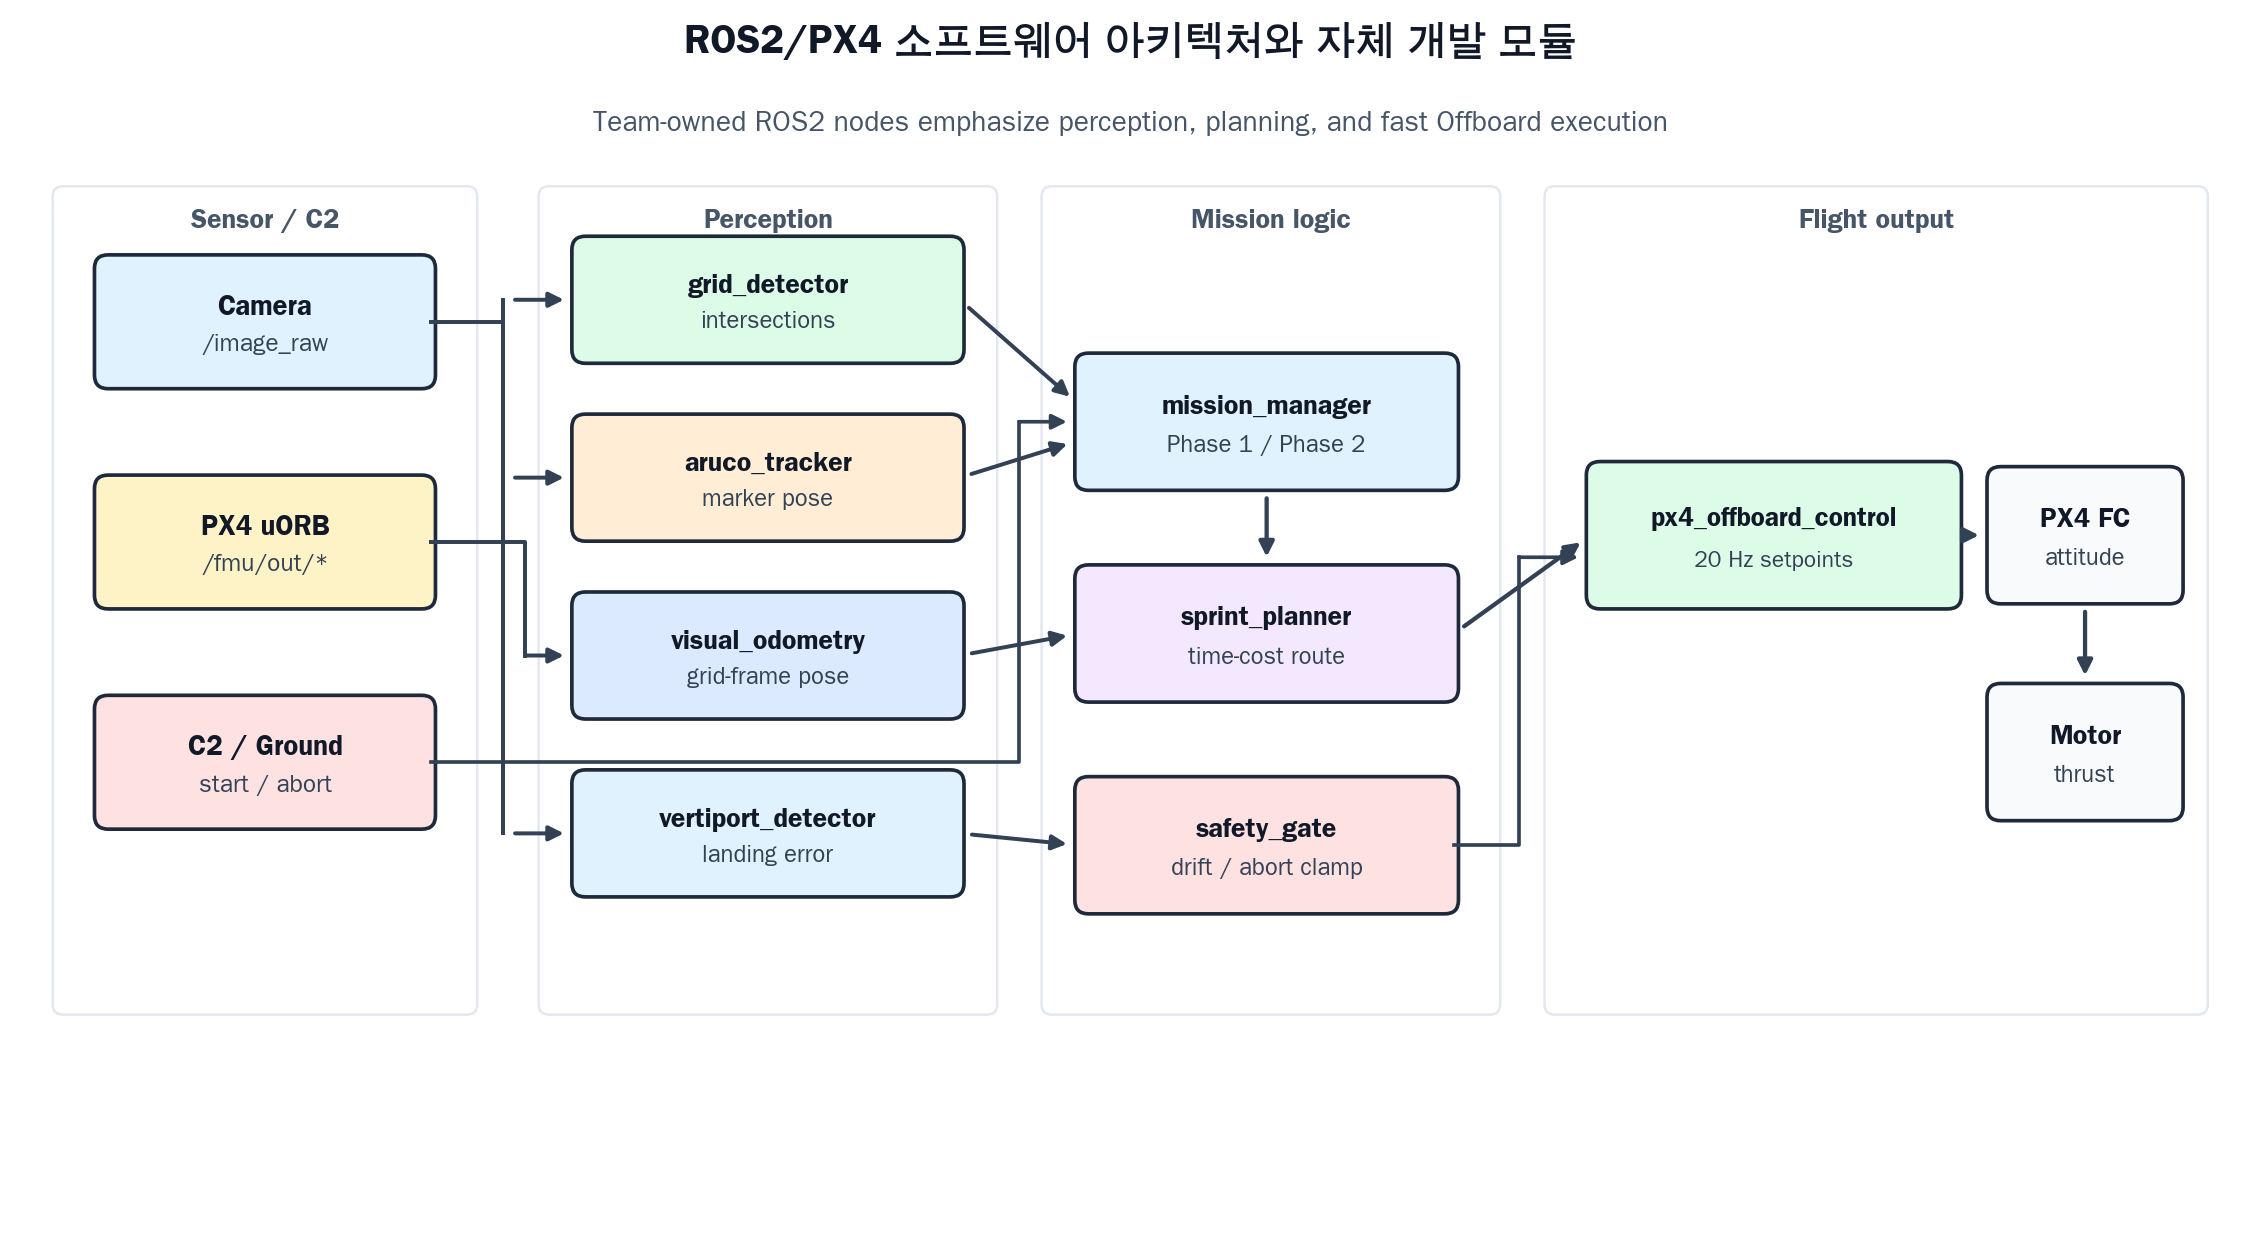
\includegraphics[width=0.92\linewidth]{fig_04_software_architecture.png}
\caption{ROS2/PX4 소프트웨어 아키텍처. 실시간 노드는 C++17, 분석 및 figure 생성은 Python 도구로 분리한다.}
\end{figure}

\begin{table}[H]
\centering
\small
\caption{현재 구현된 ROS2 C++ 패키지와 검증 범위}
\begin{tabularx}{\linewidth}{p{34mm}p{30mm}Y}
\toprule
\textbf{패키지} & \textbf{상태} & \textbf{역할}\\
\midrule
\code{grid\_detector} & 구현/단위시험 & 선분 방향 분류, collinear merge, 교차점 추출, 신뢰도 계산\\
\code{aruco\_tracker} & 구현/단위시험 & 흔들림-aware confidence filter, 후보/확정/방문 상태 관리\\
\code{visual\_odometry} & 구현/단위시험 & pixel-to-meter 변환, yaw-aware pose integration, grid snap, Home/Grid SE2 변환\\
\code{sprint\_planner} & 구현/단위시험 & 직선 구간 시간 모델, 회전/정지/호버링 비용 기반 경로 평가\\
\code{mission\_manager} & 구현/단위시험 & 미션 상태 전이, 4개 마커 완료 trigger, ID 내림차순 구조 순서, 저전압 귀환\\
\code{px4\_offboard\_control} & 구현/단위시험/SITL smoke & 모드별 속도 clamp, 가속도 rate limit, anti-sway, vision-servo setpoint\\
\code{vertiport\_detector} & 구현/단위시험 & 착륙 대상 중심 오차 추정, confidence 기반 하강 gate\\
\bottomrule
\end{tabularx}
\end{table}

\begin{lstlisting}[style=pseudo,caption={Mission manager pseudocode matching the implemented state machine},label={lst:mission}]
state <- INIT
while mission is not terminal:
    if abort_command:
        state <- ABORT
    else if battery_percent <= return_threshold and state not in landing states:
        state <- EMERGENCY_RETURN

    switch state:
        INIT:
            if mission_start: state <- TAKEOFF
        TAKEOFF:
            if takeoff_complete: state <- HOME_INIT
        HOME_INIT:
            if home_initialized: state <- GRID_SEARCH
        GRID_SEARCH:
            if confirmed_marker_count == 4: state <- RESCUE_ROUTE_PLAN
            else if marker_candidate: state <- MARKER_APPROACH
        MARKER_APPROACH:
            if perception_stable or confirmed_marker: state <- ANTI_SWAY
        ANTI_SWAY:
            if confirmed_marker:
                pending_marker <- confirmed_marker
                hover_timer.start()
                state <- HOVER_CONFIRM
        HOVER_CONFIRM:
            if hover_timer.elapsed(3.0 s):
                save_or_update_marker(pending_marker)
                state <- MARKER_SAVE
        MARKER_SAVE:
            state <- RESCUE_ROUTE_PLAN if confirmed_marker_count == 4 else GRID_SEARCH
        RESCUE_ROUTE_PLAN:
            rescue_order <- sort(marker_ids, descending)
            state <- RESCUE_VISIT
        RESCUE_VISIT:
            if target_reached for 3.0 s: advance_to_next_marker_or_RETURN_HOME()
        RETURN_HOME:
            if target_reached: state <- VERTIPORT_ACQUIRE
        VERTIPORT_ACQUIRE:
            if vertiport_acquired: state <- VISION_SERVO_LAND
        VISION_SERVO_LAND:
            if landing_complete: state <- LANDED
\end{lstlisting}

\subsection{임무 장치 및 수행 방법}

Phase 1 탐색 경로는 9 $\times$ 6 = 54개 교차점을 지나는 boustrophedon(S자) 순서다. 모든 교차점에서 정지하지 않고, 교차점은 위치 보정 체크포인트로 사용한다. 이때 ArUco detector와 confidence filter는 탐색 이동과 동시에 동작하며, 후보가 confidence 조건을 만족하는 순간에만 접근 모드로 전환한다. Fig. 6의 살구색 선은 이때 마커 중심으로 붙는 짧은 후보 접근 구간이고, 빨간 표시는 연속 이동 경로가 아니라 3초 호버링 확인 위치이다. 접근ㆍanti-swayㆍ3초 호버링은 탐색과 분리된 별도 임무가 아니라, 최초 인식 확인 조건을 만족시키기 위한 Phase 1 내부 하위 동작이다.

\begin{figure}[H]
\centering
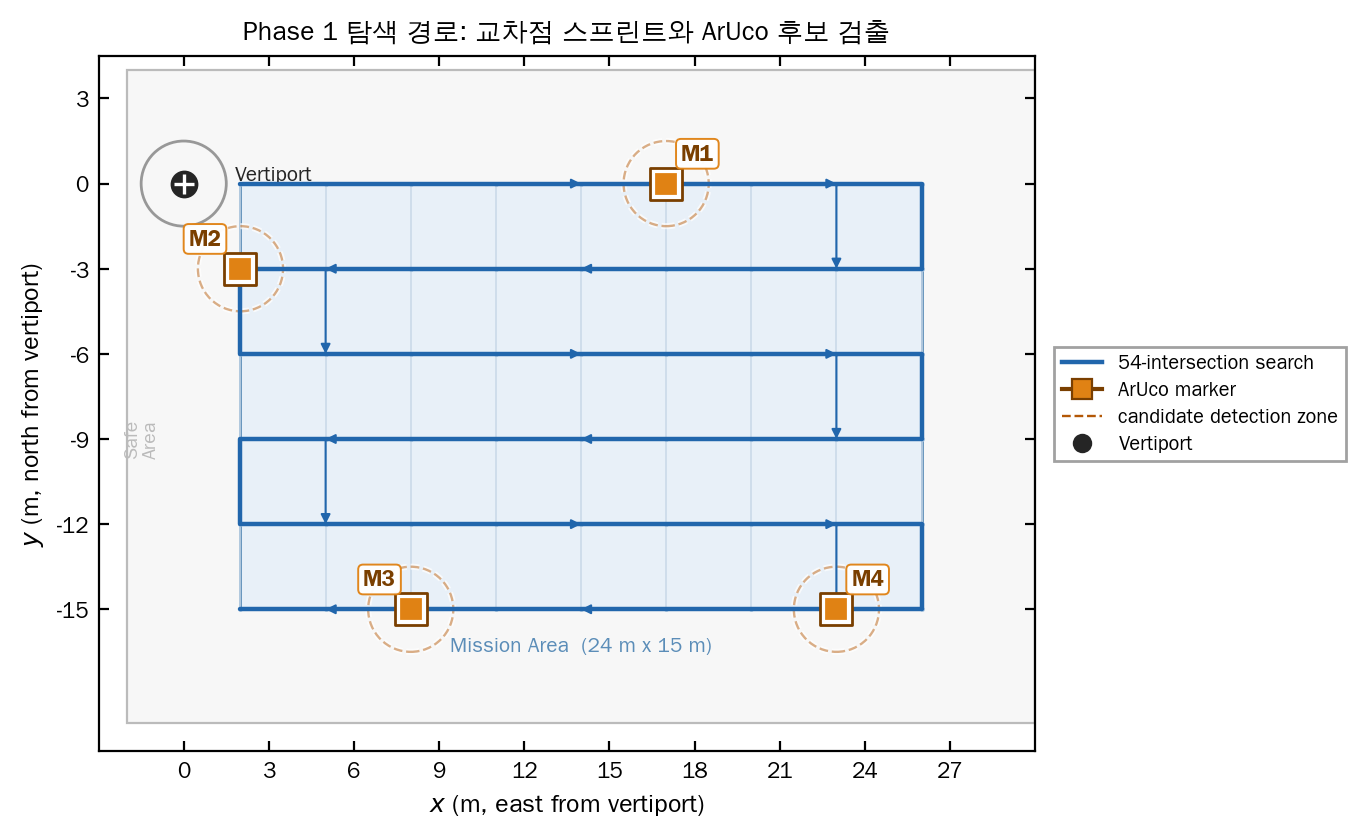
\includegraphics[width=0.80\linewidth]{fig_05_gazebo_search_path.png}
\caption{Phase 1 교차점-to-교차점 S자 탐색 경로. 하향 카메라 인식은 이동 중 계속 수행되며, 후보 확정 시에만 접근/호버링 하위 상태로 짧게 전환한다.}
\end{figure}

Phase 2 구조 경로는 저장된 마커 좌표를 ID 내림차순으로 정렬하여 직선으로 연결한다. Fig. 6에서 구조 구간이 격자선을 따라 직각으로 이동하지 않는 이유는, 이 단계의 1차 목적을 선 추종 정확도보다 \textbf{구조 대상의 신속한 재방문}으로 두기 때문이다. 즉, 구조 순서와 마커 통과 조건을 만족하는 범위 안에서 경로 길이와 감가속 시간을 줄이고, 직각 격자 경로가 만드는 불필요한 회전ㆍ정지 시간을 제거한다. 정확도 위험은 저장 좌표 접근 오차, 재검출 실패 가능성, 중심 정렬 오차를 기준으로 관리하며, 각 구조 마커 종단부에서 ArUco 재검출ㆍvision servo 정렬ㆍ3초 호버링을 수행해 보상한다.

현재 headless 기록과 비용 모델은 구조/귀환 스프린트 속도를 10m/s로 두었지만, 향후 목표는 동일 구조 경로를 20m/s급으로 확장하는 것이다. 다만 속도 $v$가 증가하면 마커가 카메라 시야의 유효 검출 폭 $L_{\mathrm{vis}}$ 안에 머무는 프레임 수가
\begin{equation}
N_{\mathrm{frame}}(v)=\frac{f_{\mathrm{cam}}L_{\mathrm{vis}}}{v}
\end{equation}
로 감소한다. 예를 들어 $f_{\mathrm{cam}}=60$fps, $L_{\mathrm{vis}}=3$m이면 10m/s에서는 약 18프레임, 20m/s에서는 약 9프레임만 확보된다. 따라서 20m/s 확장 단계에서는 motion blur 억제, 노출 시간 최적화, 예측 기반 ROI cropping, temporal confidence filter, 접근 반경의 adaptive slowdown을 함께 최적화하여 고속화로 인한 인식 불안정성을 보상한다. 각 구조 마커에서는 ArUco를 재검출하고 중심 오차가 충분히 작을 때 3초 호버링을 수행한다.

\begin{figure}[H]
\centering
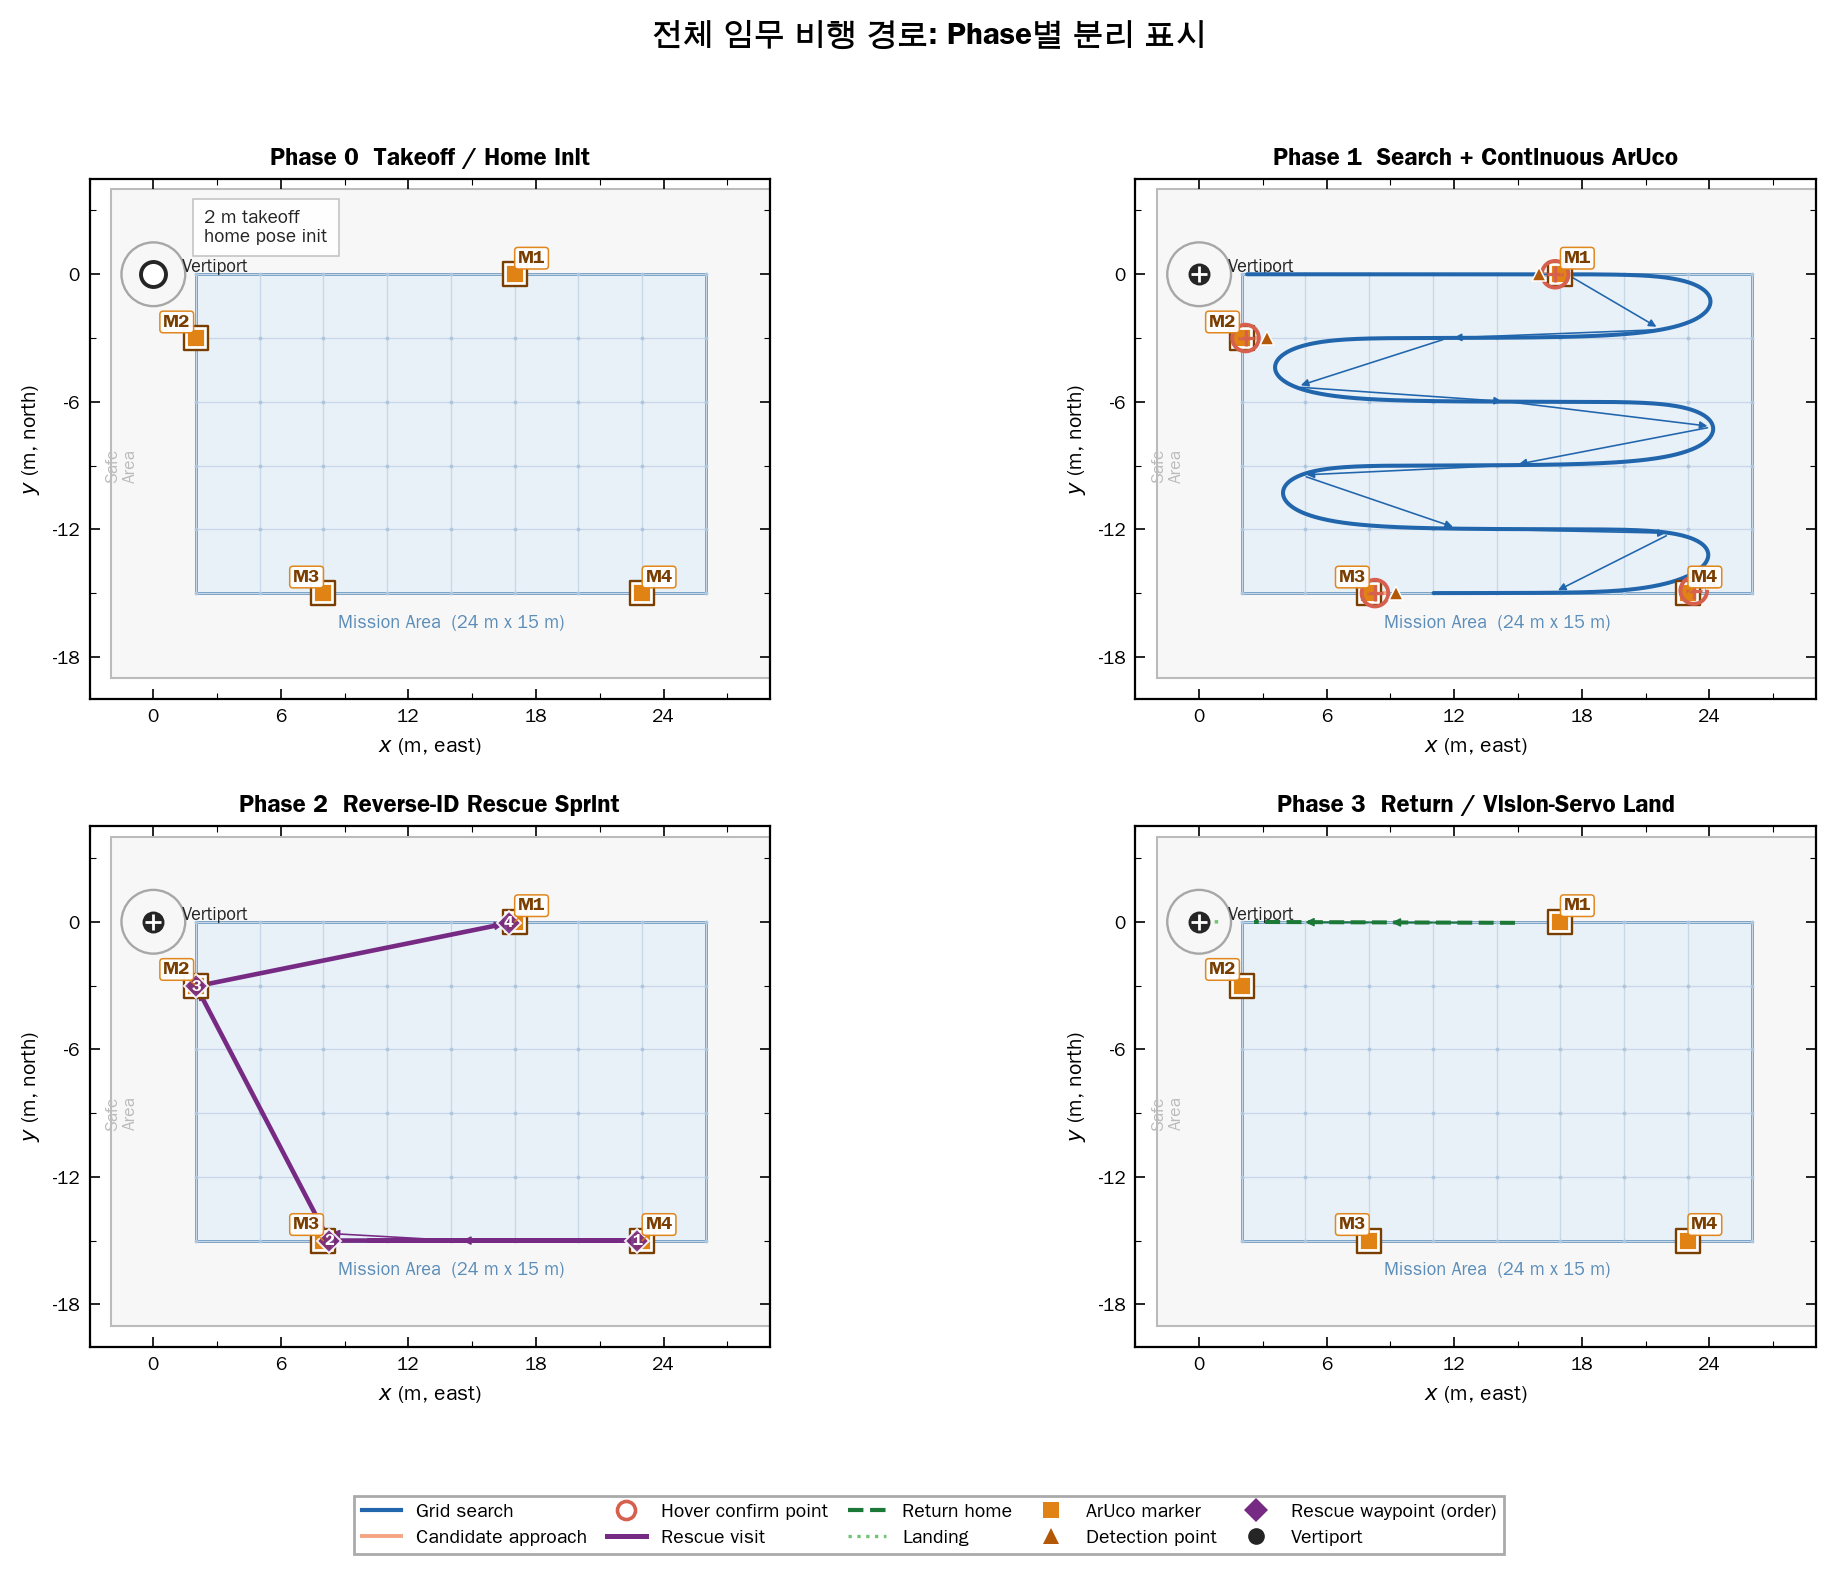
\includegraphics[width=0.96\linewidth]{fig_06_gazebo_mission_path.png}
\caption{Phase별 전체 미션 경로와 구조 방문 순서. Phase 1은 탐색 이동과 연속 ArUco 인식을 병행하며, 살구색은 후보 확정 후 마커 중심으로 붙는 짧은 접근 구간, 빨간 원은 3초 호버링 확인 위치를 뜻한다. Phase 2는 ID 역순 직선 구조 스프린트, Phase 3은 귀환 및 vision-servo 착륙을 나타낸다.}
\end{figure}

\textbf{Mission-cost sweep.} 아래 결과는 실제 완주 시간이 아니라, Gazebo world와 동일한 54개 교차점 후보에서 600개 랜덤 마커 배치(seed 0--599)를 생성하여 계산한 경로 비용 모델 결과이다. 모델 조건은 Phase 1 탐색 10m/s, 구조/귀환 10m/s, 탐색 호버링 12초, 구조 호버링 12초, Phase 0 1.5초, 착륙 4초이다. 전체 시간은 최소 40.7초, 중앙값 50.5초, 최대 57.9초였다. 현재 Gazebo seed 310은 spread 유형이며 52/54번째 교차점에서 4개 마커를 모두 발견하고, 총 시간은 53.6초로 계산된다.

\begin{table}[H]
\centering
\small
\caption{600개 랜덤 ArUco 배치 mission-cost sweep 요약}
\begin{tabular}{lrrrrrr}
\toprule
\textbf{배치 유형} & \textbf{개수} & \textbf{중앙 총시간} & \textbf{중앙 Phase1} & \textbf{중앙 Phase2} & \textbf{탐색거리} & \textbf{구조+귀환거리}\\
\midrule
clustered & 327 & 49.4s & 25.9s & 16.5s & 134.0m & 58.1m\\
mixed     & 216 & 51.2s & 26.8s & 17.2s & 143.0m & 63.1m\\
spread    &  57 & 52.4s & 27.1s & 18.3s & 146.0m & 73.8m\\
\bottomrule
\end{tabular}
\end{table}

\begin{figure}[H]
\centering
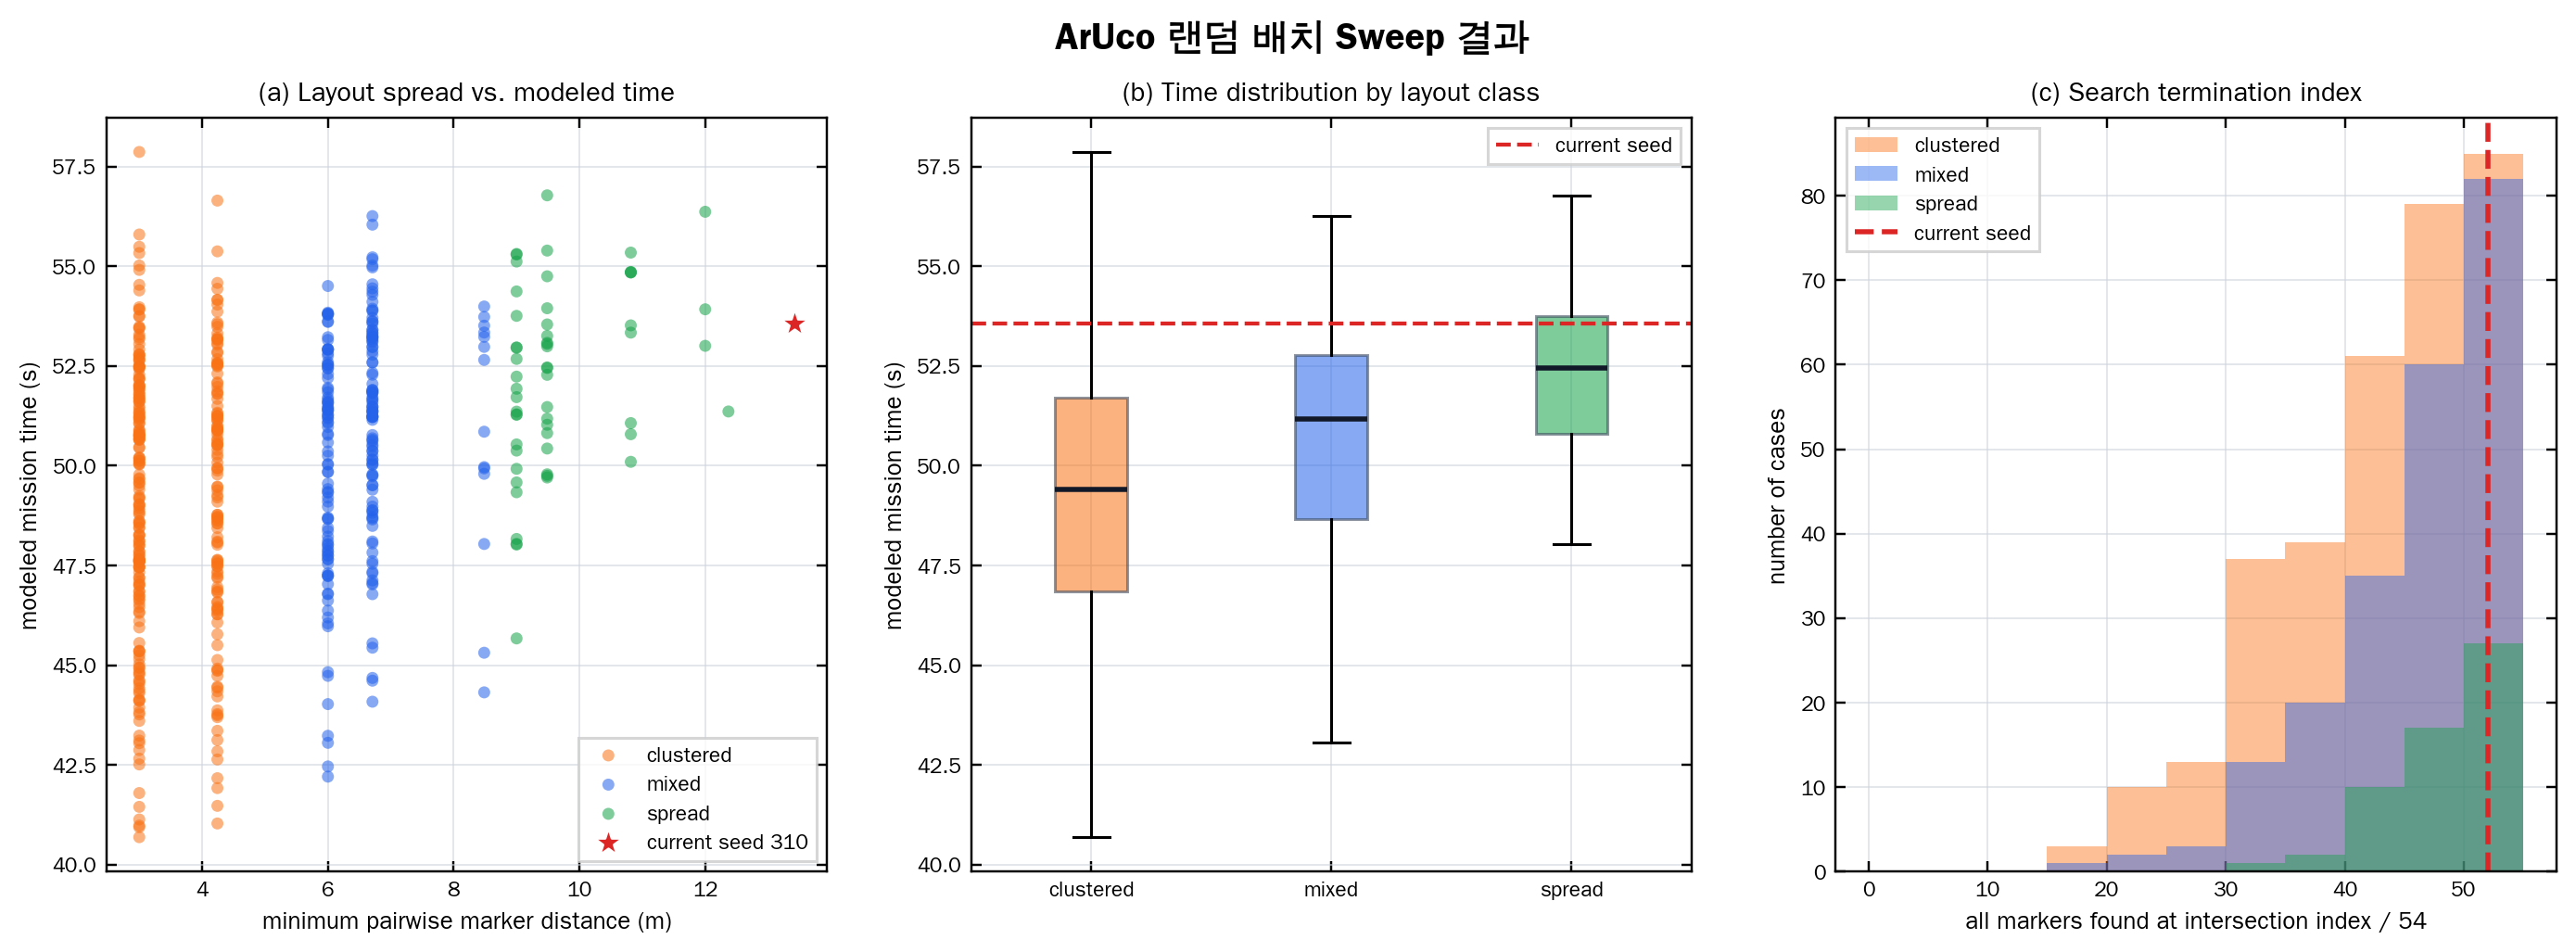
\includegraphics[width=0.94\linewidth]{fig_11_marker_sweep_results.png}
\caption{600개 랜덤 마커 배치에 대한 mission-cost sweep. 군집/혼합/분산 배치와 seed 310의 위치를 비교한다.}
\end{figure}

\begin{figure}[H]
\centering
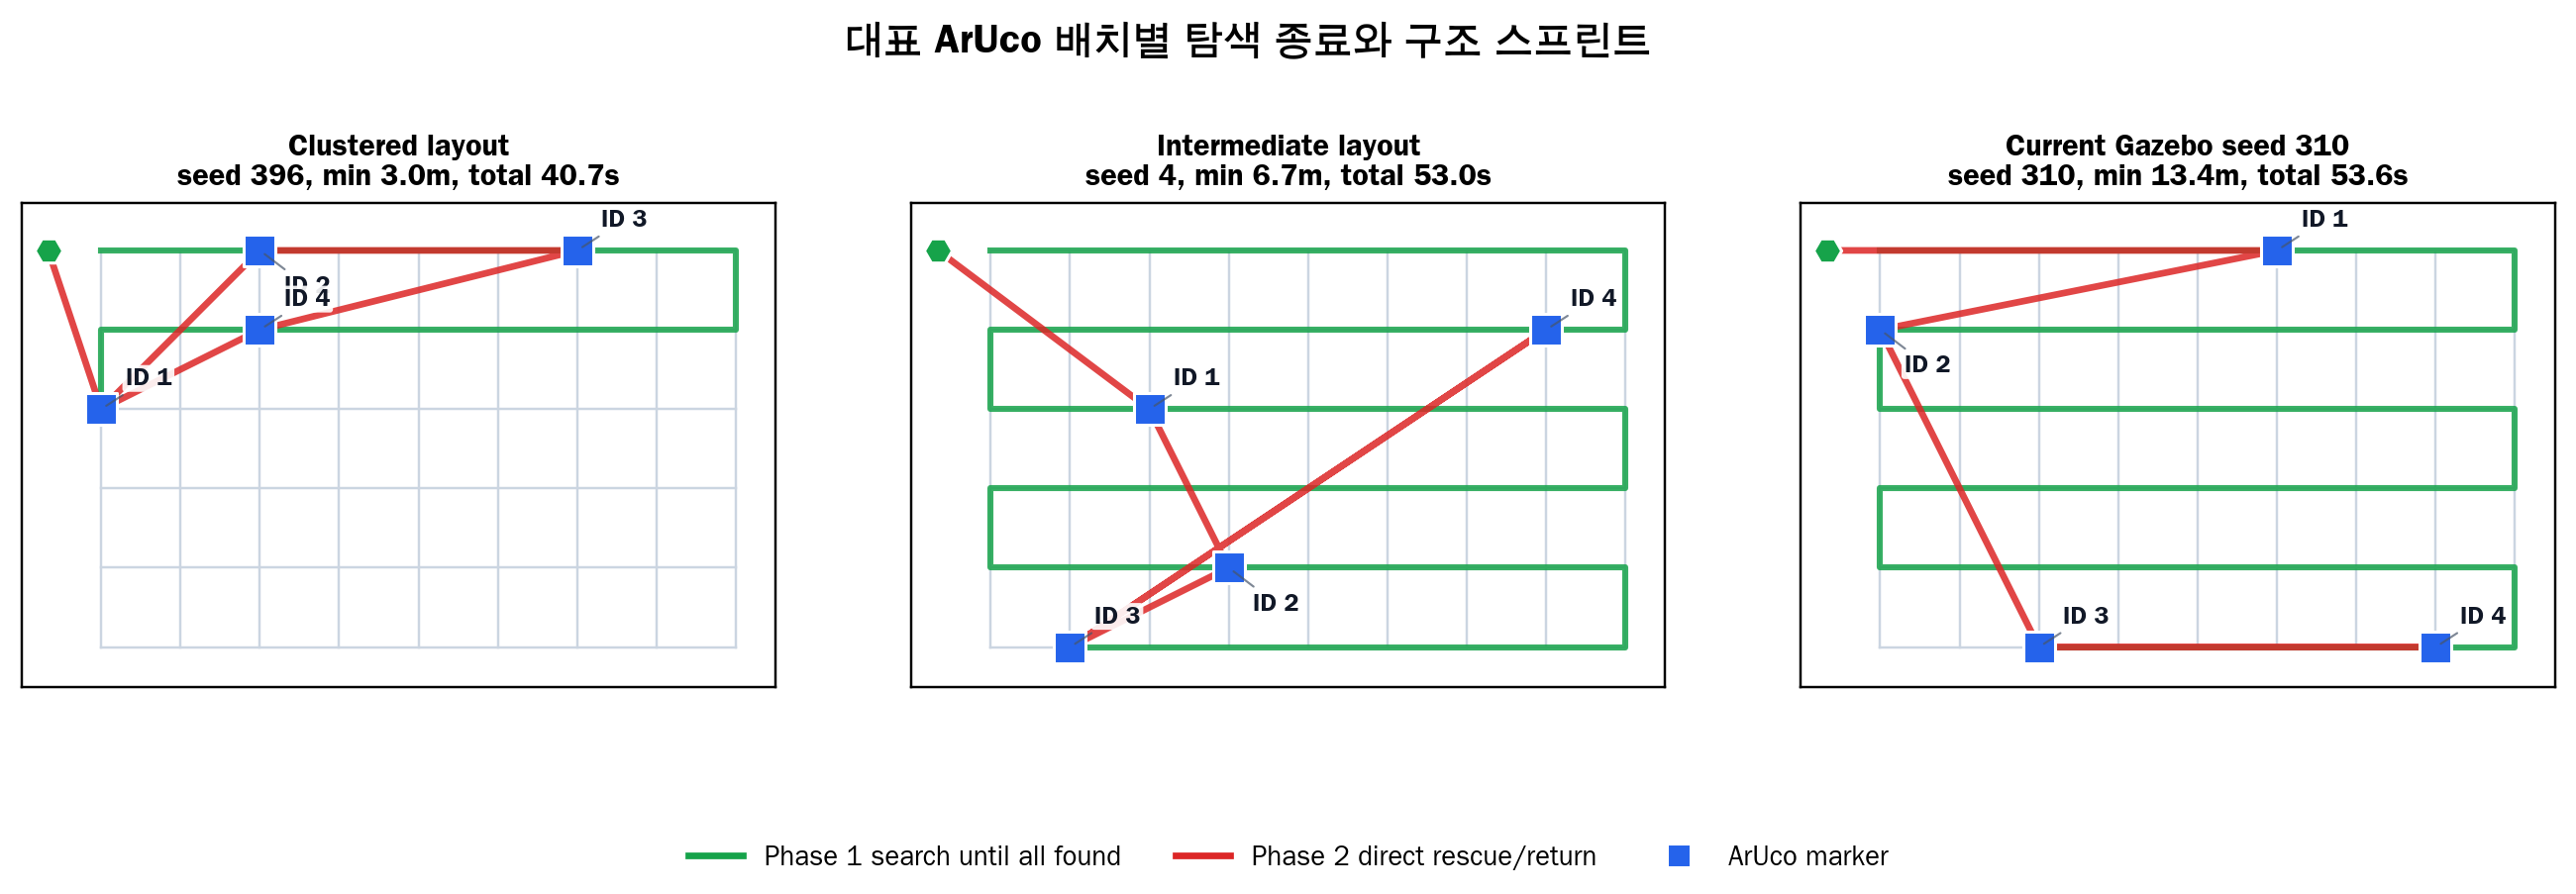
\includegraphics[width=0.94\linewidth]{fig_12_marker_layout_cases.png}
\caption{대표 마커 배치별 탐색 종료 지점과 구조/귀환 경로 비교.}
\end{figure}

Phase 1 속도를 5/7/10m/s로 바꾸어 동일한 600개 배치를 계산하면 중앙값은 64.5초, 56.5초, 50.5초로 감소한다. 반면 60fps 카메라에서 마커가 가시 구간 3m 안에 머무는 프레임 수는 36.0, 25.7, 18.0프레임으로 감소한다. 따라서 10m/s 모델은 시간상 유리하지만, 실제 적용 속도는 고속 ArUco 검출 성공률 실험으로 보정해야 한다.

\begin{table}[H]
\centering
\small
\caption{Phase 1 속도 sweep: 시간 이득과 인식 노출 trade-off}
\begin{tabular}{rrrrrrr}
\toprule
\textbf{속도} & \textbf{최소} & \textbf{평균} & \textbf{중앙값} & \textbf{최대} & \textbf{seed 310} & \textbf{60fps 프레임}\\
\midrule
5m/s  & 45.3s & 63.1s & 64.5s & 73.7s & 69.1s & 36.0\\
7m/s  & 42.8s & 55.6s & 56.5s & 64.6s & 60.2s & 25.7\\
10m/s & 40.7s & 49.9s & 50.5s & 57.9s & 53.6s & 18.0\\
\bottomrule
\end{tabular}
\end{table}

\begin{figure}[H]
\centering
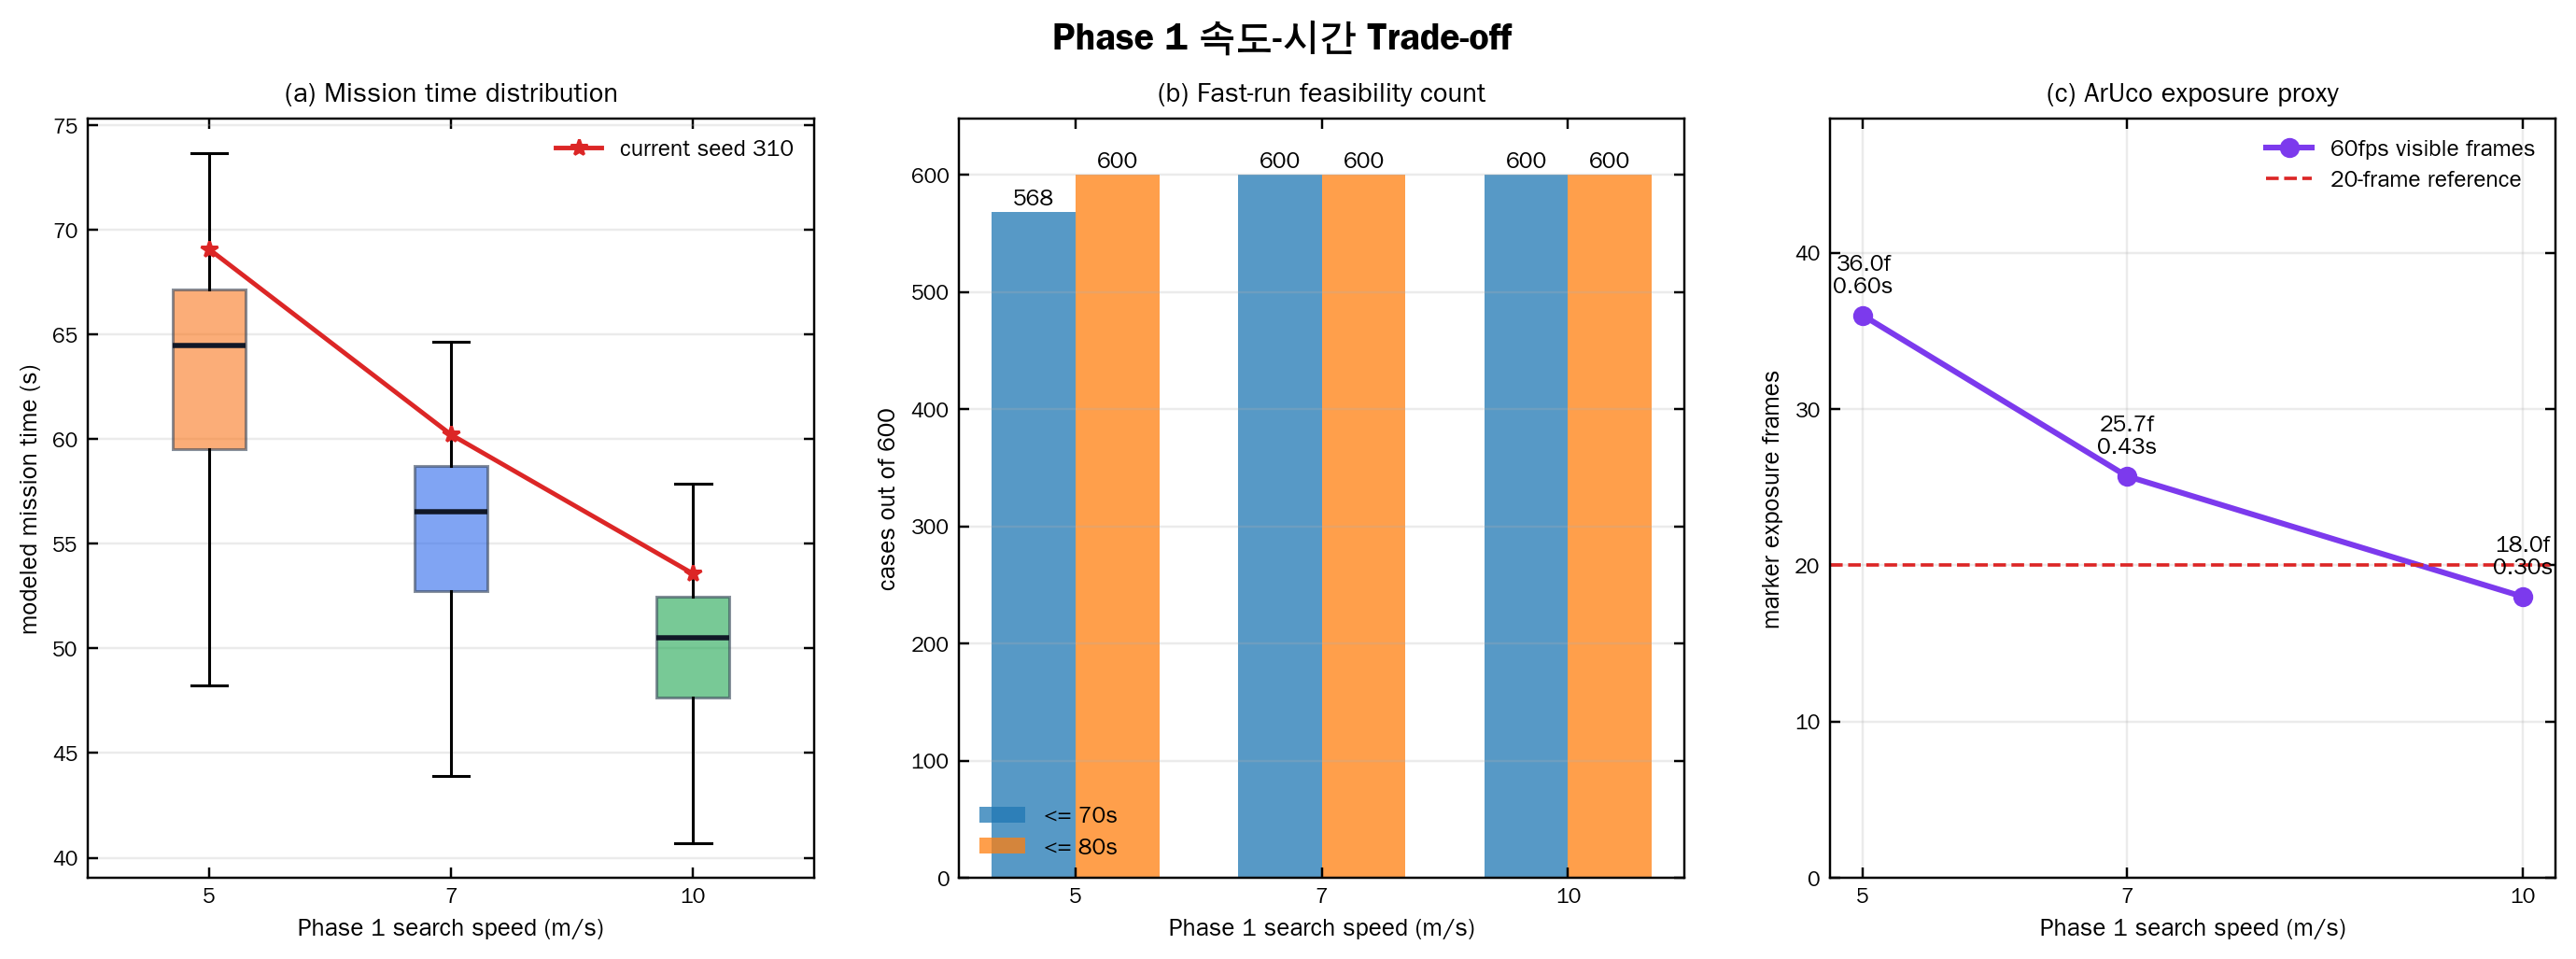
\includegraphics[width=0.94\linewidth]{fig_13_phase1_speed_tradeoff.png}
\caption{Phase 1 속도 변화에 따른 임무 시간과 마커 노출 프레임 수.}
\end{figure}

\subsection{구성품의 적정성}

구성품 선정의 핵심 기준은 고속 비전 항법과 PX4 Offboard 제어를 안정적으로 수행할 수 있는가이다. 본 계획의 자체 개발성은 기체 프레임 제작보다 인식, 항법, 미션 상태 기계, 경로 비용 모델, 안전 gate에 있다.

\begin{table}[H]
\centering
\small
\caption{구성품 선정 기준}
\begin{tabularx}{\linewidth}{p{35mm}Y}
\toprule
\textbf{구성품} & \textbf{기술적 적정성}\\
\midrule
PX4/ArduPilot 지원 FC & 저수준 자세 안정화와 failsafe를 검증된 비행제어기가 담당하고, Companion Computer가 고수준 setpoint를 생성\\
하향 글로벌 셔터 카메라 & 고속 이동 중 rolling shutter 왜곡을 줄여 Optical Flow, 격자 교차점, ArUco 인식률 확보\\
ToF 거리 센서 & 2m 고도 유지와 pixel-to-meter 스케일 보정의 기준 센서\\
Companion Computer & OpenCV와 ROS2 C++ 노드, PX4 bridge를 동시에 실행할 연산 여유 확보\\
독립 5V DC-DC 전원 & 급가속/급감속 중 Companion Computer 리셋과 Offboard setpoint 단절 방지\\
통신 모듈/C2 & 미션 시작, abort, 상태 모니터링, 시험 중 안전 개입\\
\bottomrule
\end{tabularx}
\end{table}

\subsection{지상 및 비행 시험 계획}

시험 환경은 Ubuntu 24.04, ROS2 Jazzy, Gazebo Harmonic, PX4 SITL, Micro XRCE-DDS Agent, ROS2-PX4 bridge로 구성한다. 현재 C++ core 단위시험, Gazebo/PX4 smoke check, ROS2 headless 전체 미션 기록을 확보했다. Headless 기록은 \code{mock\_sensors.py}와 \code{gz\_drone\_sim.py} 기반의 통합 실행이므로, PX4 동역학까지 포함한 전체 미션 성공과는 구분해 해석한다.

\begin{table}[H]
\centering
\small
\caption{현재 검증 현황과 남은 검증 항목}
\begin{tabularx}{\linewidth}{p{34mm}p{20mm}Y}
\toprule
\textbf{항목} & \textbf{상태} & \textbf{근거 / 성공 기준}\\
\midrule
C++ core 단위시험 & 완료 & planner, grid, aruco, odometry, mission, control, vertiport 테스트 존재\\
PX4 SITL 빌드/실행 & 완료 & \code{gz\_x500\_mono\_cam\_down} 월드 실행 및 PX4 sensor topics 확인\\
Offboard 진입 smoke & 완료 & \code{/mission/start} 후 armed/offboard 진입 확인\\
Headless 전체 미션 rosbag & 완료 & 57.500초 bag, LANDED 52.69초, pose 1,437개, planner profile 576개, 목표 속도 10.0m/s\\
고속 ArUco 성공률 & 예정 & 4/6/8/10m/s 조건별 ID 확정률 측정\\
Optical Flow 오차 & 예정 & 2m 고도에서 3m edge 이동 후 snap 전/후 오차 측정\\
PX4/Gazebo 전체 미션 완주 & 예정 & 이륙, 4마커 탐색/저장, 역순 구조, 귀환, 착륙을 PX4 SITL 동역학으로 연속 수행\\
\bottomrule
\end{tabularx}
\end{table}

\begin{figure}[H]
\centering
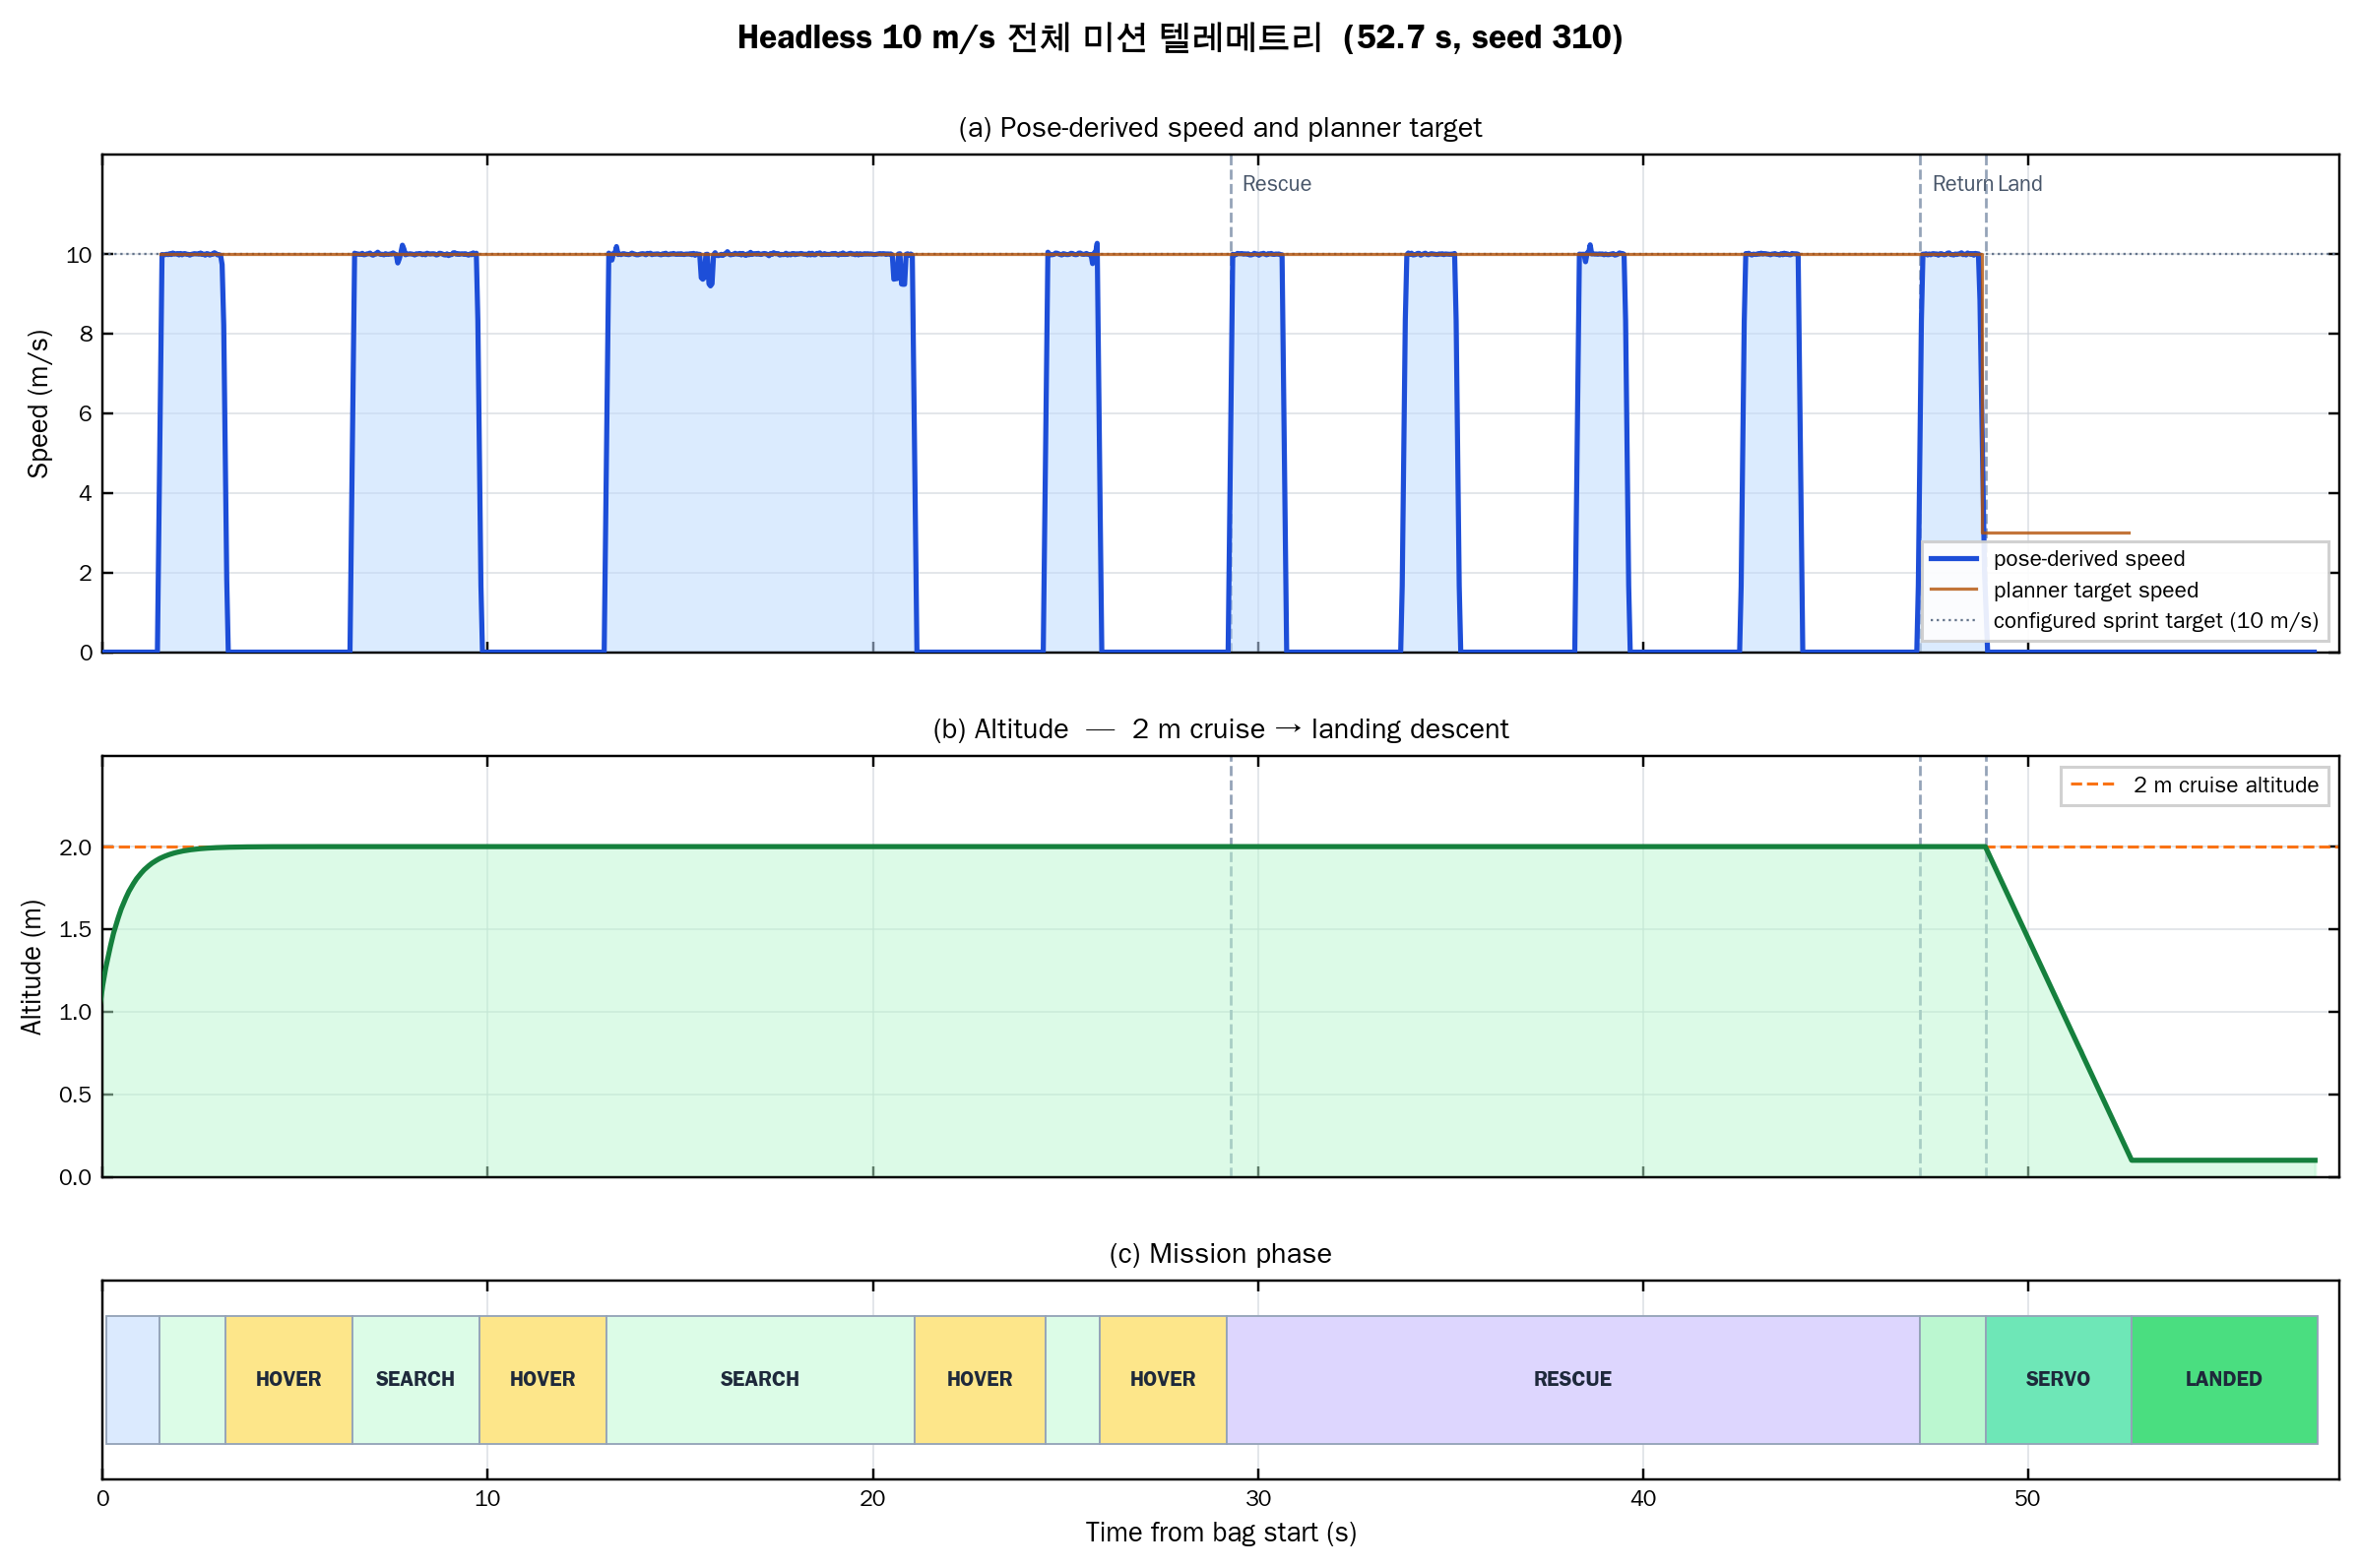
\includegraphics[width=0.95\linewidth]{fig_08_gazebo_telemetry.png}
\caption{Headless ROS2 10m/s 전체 미션 텔레메트리. Planner target speed는 10.0m/s까지 도달하고, pose 기반 지상속도 p95는 약 10m/s이다. 본 그림은 PX4/Gazebo 전체 동역학 검증이 아니라, 상태 전이와 경로 생성 로직의 headless 통합 기록이다.}
\end{figure}

\section{시스템 설계 및 제작상의 특장점}
\subsection{시스템 구현에서의 창의성}

본 시스템의 창의성은 격자 경기장을 저속 라인 추종 대상이 아니라 \textbf{3m 간격 위치 보정 기준을 가진 고속 항법 공간}으로 해석한 데 있다. Fig. 9는 일반적인 라인 트레이싱 중심 접근과 본 팀의 교차점 스프린트 전략을 비교한다.

\begin{figure}[H]
\centering
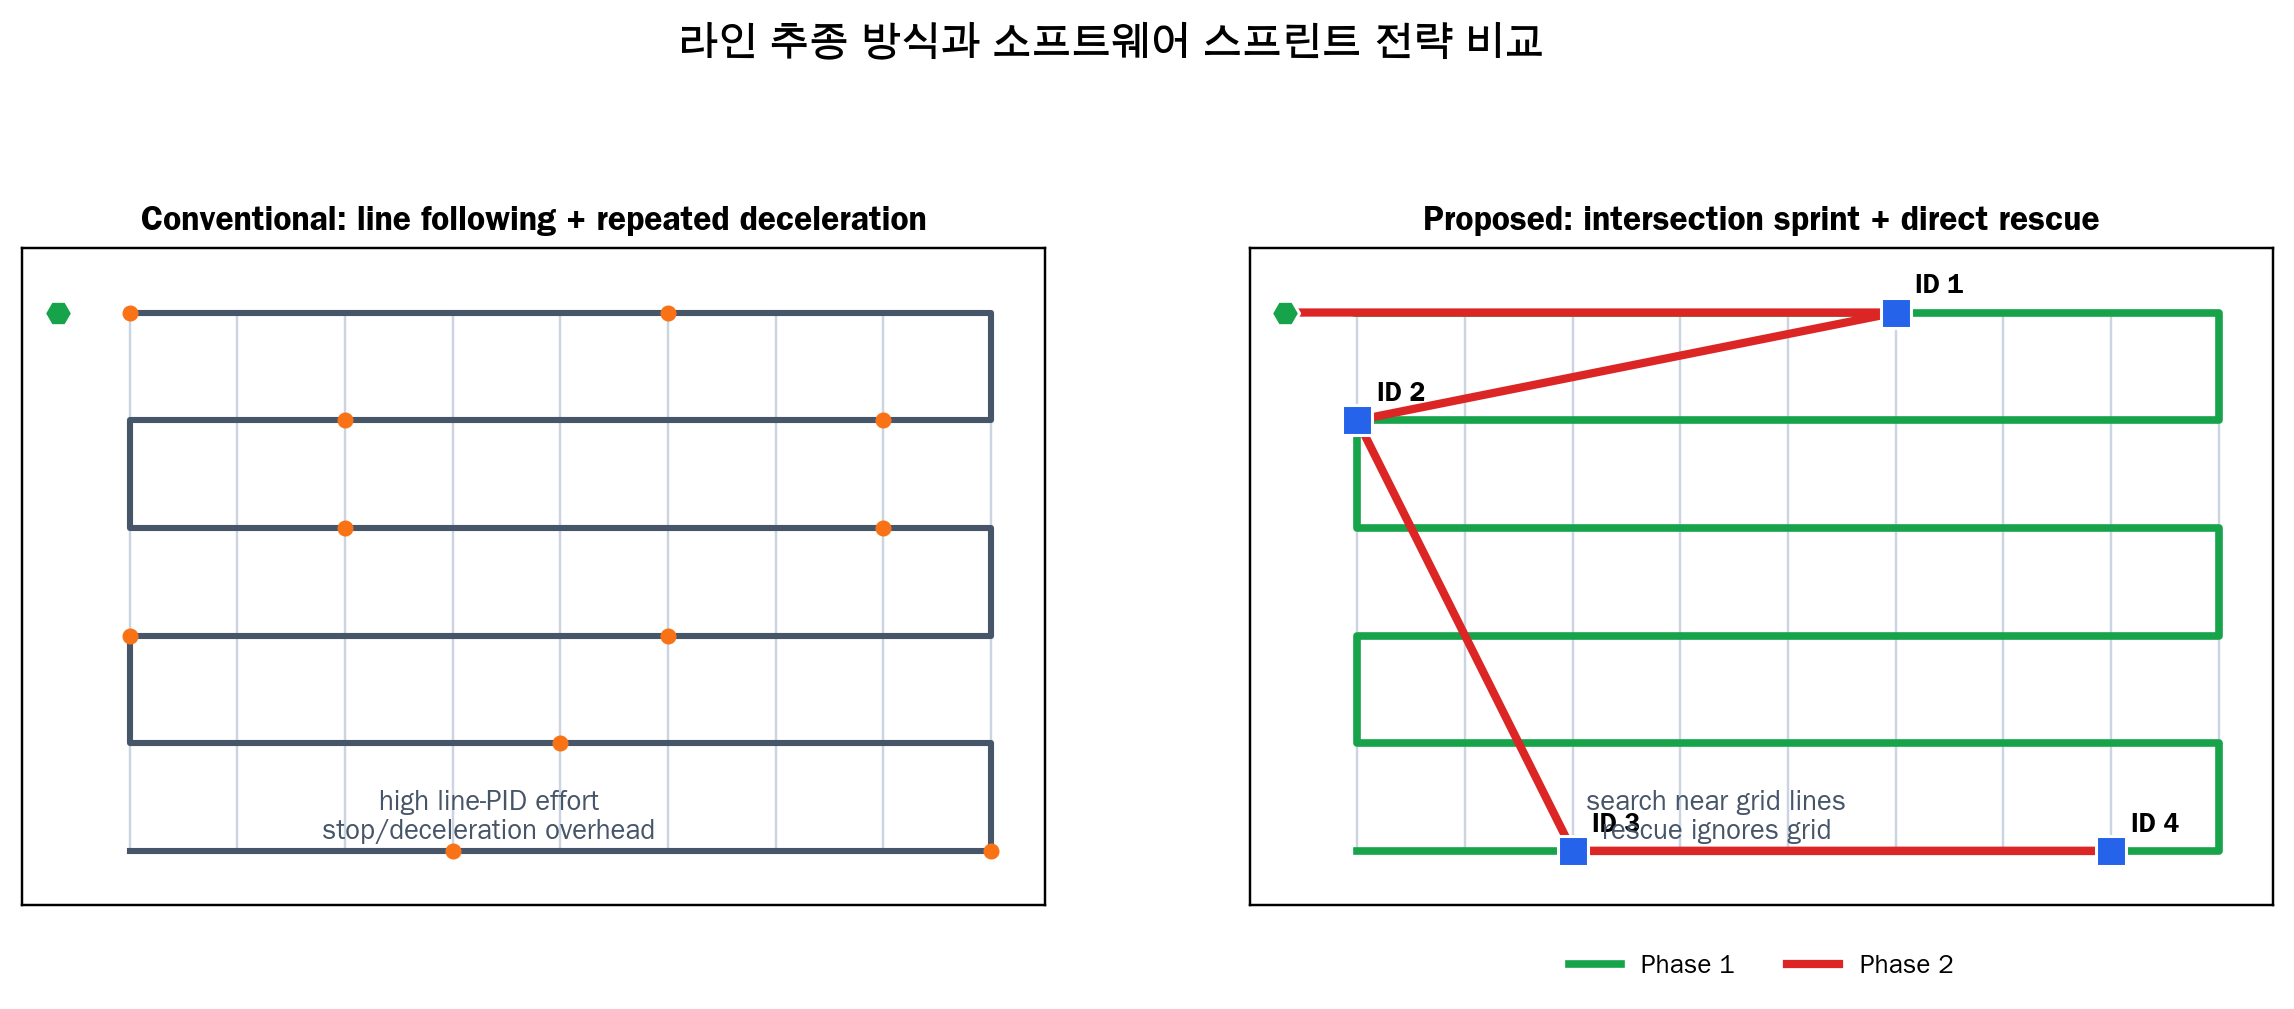
\includegraphics[width=0.92\linewidth]{fig_09_strategy_comparison.png}
\caption{일반 라인 트레이싱 접근과 교차점 스프린트/직선 구조 전략 비교.}
\end{figure}

\begin{enumerate}
\item \textbf{교차점 snap 항법:} Optical Flow 적분 drift를 3m 간격 교차점에서 주기적으로 보정한다.
\item \textbf{탐색/구조 분리:} 탐색은 격자 기반, 구조는 ID 역순 직선 스프린트로 처리한다.
\item \textbf{마커 후보 기반 감속:} 모든 교차점에서 멈추지 않고, 후보가 확인될 때만 접근ㆍanti-swayㆍhover를 수행한다.
\item \textbf{시간 기반 경로 평가:} 거리뿐 아니라 가속/감속, 회전, 정지, 호버링, 재검출 안정성을 함께 비교한다.
\item \textbf{Perception-aware control:} 마커 후보, 흔들림 metric, 버티포트 중심 오차가 제어 모드 전환에 직접 반영된다.
\end{enumerate}

\begin{table}[H]
\centering
\small
\caption{채점 항목별 대응 전략}
\begin{tabularx}{\linewidth}{p{31mm}p{16mm}p{22mm}Y}
\toprule
\textbf{채점 항목} & \textbf{배점} & \textbf{목표} & \textbf{대응 기술}\\
\midrule
경로점 위치 추정 & 120 & 상 등급 & Optical Flow + 교차점 snap + 마커 confidence 저장\\
ArUco ID 식별 & 40 & 전량 확보 & OpenCV ArUco 검출, ID별 누적 filter\\
고도 유지 & 30 & 상 등급 & PX4 고도 제어, ToF scale 보정\\
구획선 이탈 & 40 & 부분--상향 목표 & 교차점 직선 경로로 격자선 근처 이동, drift 과다 시 재획득\\
구조 방문 순서 & 40 & 전량 확보 & ID 내림차순 rescue order 생성\\
구조 통과 정확도 & 80 & 상 등급 & 저장 좌표 접근 후 ArUco 재검출, vision servo 중심 정렬\\
임무 수행 시간 & 100 & 상위권 목표 & Phase 1 정지 최소화, Phase 2/3 직선 스프린트\\
자체 개발 가산 & 50 & 최대 확보 & ROS2 C++ 인식/항법/계획/제어/안전 모듈 자체 구현\\
\bottomrule
\end{tabularx}
\end{table}

\section{안전장치에 대한 설명}
\subsection{안전장치의 구성 및 성능}

고속 스프린트 전략은 안전 envelope 없이는 성립하지 않는다. 제어기는 mission state를 control mode로 매핑하고, 각 mode별 수평/수직 속도, 가속도, jerk, tilt 제한을 적용한다. 예를 들어 SPRINT 모드는 큰 수평 속도를 허용하지만, APPROACH, ANTI\_SWAY, HOVER\_CONFIRM, VISION\_SERVO에서는 속도를 강하게 제한한다.

\begin{table}[H]
\centering
\small
\caption{안전 기능 구성}
\begin{tabularx}{\linewidth}{p{35mm}Y}
\toprule
\textbf{안전 기능} & \textbf{설명}\\
\midrule
C2 Mission Abort & 지상국에서 즉시 미션 중단, 감속, 호버 또는 착륙 명령\\
PX4 failsafe & Offboard setpoint 단절, 통신 이상, 센서 이상 시 FC 계층 failsafe 사용\\
저전압 귀환 & battery percent가 20\% 이하이면 \code{EMERGENCY\_RETURN} 전환\\
속도/가속도 envelope & mode별 \code{v\_max}, \code{a\_max}, jerk, tilt 제한 적용\\
흔들림 억제 & sway metric이 임계값을 넘으면 \code{ANTI\_SWAY}로 전환\\
마커/버티포트 재획득 & confidence 부족 시 감속, 주변 탐색, 하강 gate 차단\\
착륙 gate & 중심 오차, 검출 confidence, 수평 속도 조건 충족 시에만 하강\\
\bottomrule
\end{tabularx}
\end{table}

\subsection{안전장치의 기술적 적정성}

마커 또는 버티포트 접근 시 필요한 제동 거리는 $d_b(v)=v^2/(2b)$로 계산한다. 접근 반경은 최소 반경 $r_{\min}$, 제동 거리, 인식 안정 거리를 모두 고려한다.
\begin{equation}
r_{\mathrm{approach}}=\max(r_{\min}, d_b(v)+r_{\mathrm{detect}}).
\end{equation}
버티포트 착륙에서는 픽셀 중심 오차를 지상 거리 오차로 변환하고, confidence와 정렬 오차가 기준을 만족할 때만 하강한다.
\begin{equation}
\mathbf{e}_{xy}=
s(h)
\begin{bmatrix}
u_c-W/2\\
v_c-H/2
\end{bmatrix},
\qquad
\mathrm{descend}=
(c\ge c_{\mathrm{th}})\land(\lVert\mathbf{e}_{xy}\rVert\le e_{\mathrm{th}}).
\end{equation}

\begin{lstlisting}[style=pseudo,caption={Safety supervisor pseudocode},label={lst:safety}]
if abort_command:
    publish HOLD or LAND command
if offboard_setpoint_timeout:
    rely on PX4 failsafe and stop mission progression
if battery_percent <= 20:
    state <- EMERGENCY_RETURN
if sway_metric > sway_threshold and mode in {SPRINT, APPROACH}:
    mode <- ANTI_SWAY
if localization_drift > drift_limit:
    reduce speed and reacquire nearest grid intersection
if vertiport_confidence < threshold:
    block descent
if center_error < align_threshold and velocity_xy < limit:
    allow controlled descent
\end{lstlisting}

\begin{figure}[H]
\centering
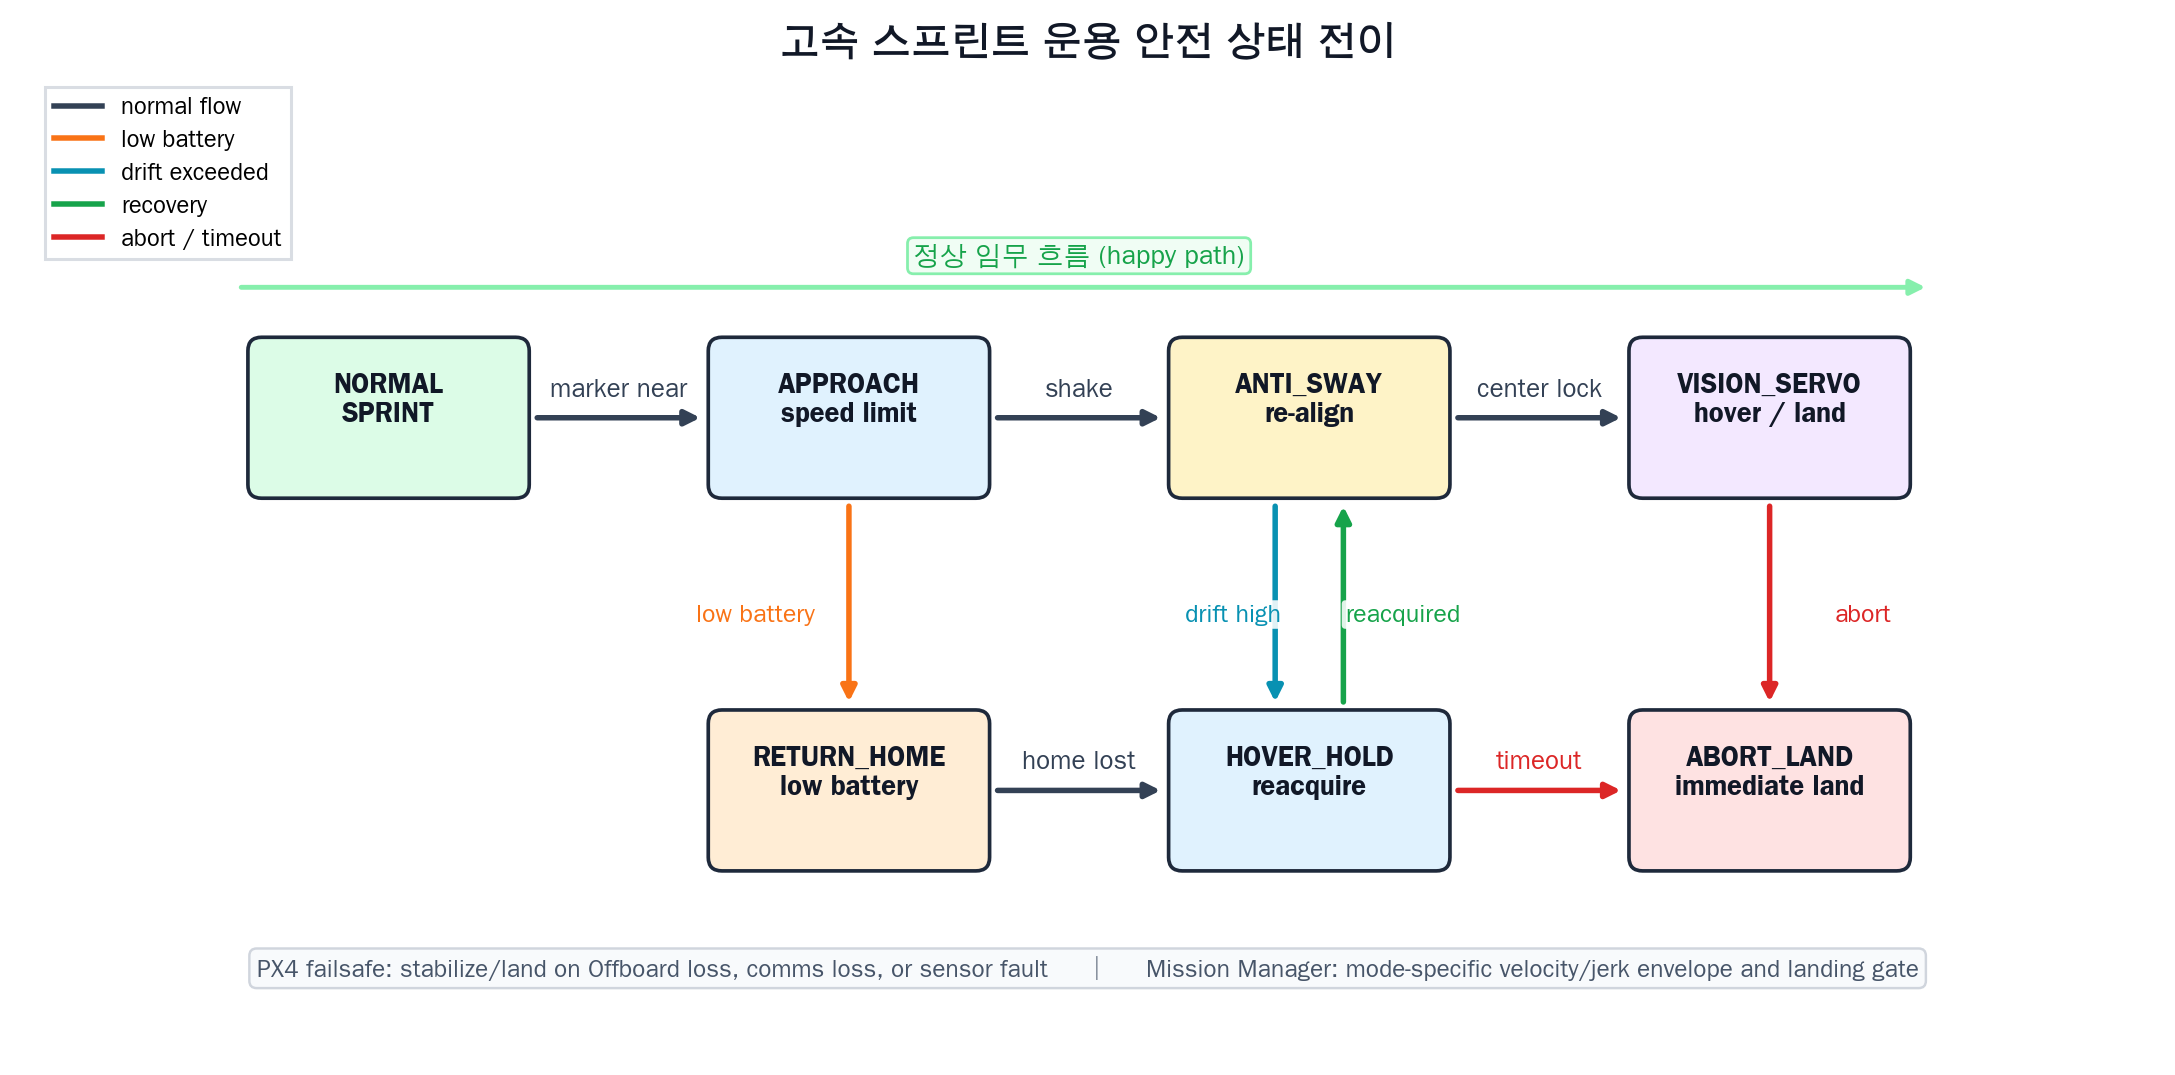
\includegraphics[width=0.92\linewidth]{fig_10_safety_state_machine.png}
\caption{고속 스프린트 전략을 위한 안전 상태 전이도.}
\end{figure}

\subsection{안전장치의 시뮬레이션 또는 실제 작동}

현재 확인된 자료는 C++ 단위시험, Gazebo/PX4/ROS2 smoke run, 10m/s 목표 headless 전체 미션 기록이다. Headless 기록은 이륙부터 \code{LANDED}까지의 상태 전이를 검증하지만, 실제 기체 또는 PX4 동역학 전체 검증은 아니다. 다음 단계에서는 동일 환경에서 Offboard setpoint 중단, 저전압 입력, drift 과다 입력, 마커 재검출 실패, 착륙 gate 실패 조건을 주입해 안전장치 작동을 반복 검증한다.

\begin{table}[H]
\centering
\small
\caption{안전장치 시험 계획}
\begin{tabularx}{\linewidth}{p{34mm}p{22mm}Y}
\toprule
\textbf{시험 항목} & \textbf{상태} & \textbf{성공 기준}\\
\midrule
Mission abort & 예정 & 즉시 속도 0 또는 착륙 mode 전환\\
Offboard setpoint timeout & 예정 & PX4 failsafe 또는 HOLD/LAND 진입 확인\\
저전압 귀환 & 구현/시험 예정 & 20\% 이하 입력 시 \code{EMERGENCY\_RETURN}\\
Sway 과다 & 단위시험 완료 & \code{SPRINT}에서 \code{ANTI\_SWAY} 전환 및 속도 제한\\
착륙 gate & 단위시험 완료 & 중심 오차/검출 조건 미충족 시 하강 금지\\
전체 통합 안전 시나리오 & 예정 & Gazebo/PX4에서 이벤트 주입 후 상태 전이 기록\\
\bottomrule
\end{tabularx}
\end{table}

\end{document}
